% Created by tikzDevice version 0.12.3.1 on 2023-02-07 11:42:22
% !TEX encoding = UTF-8 Unicode
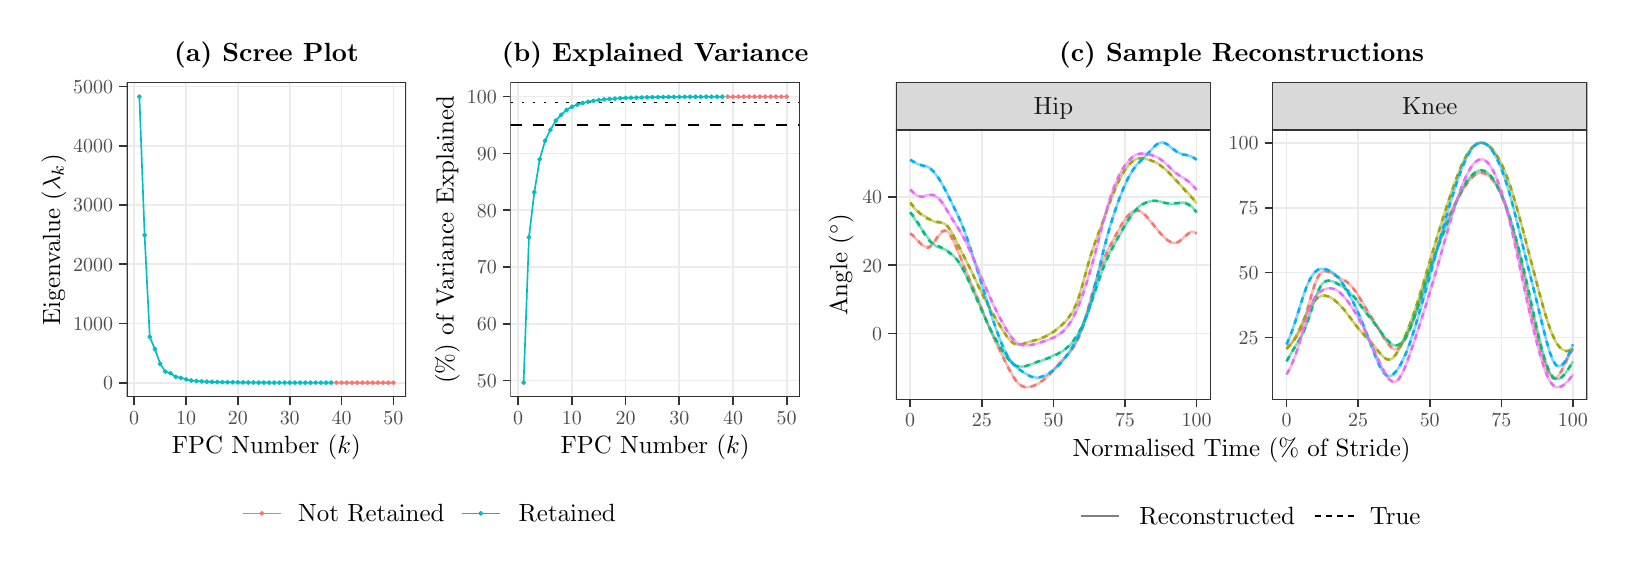
\begin{tikzpicture}[x=1pt,y=1pt]
\definecolor{fillColor}{RGB}{255,255,255}
\path[use as bounding box,fill=fillColor,fill opacity=0.00] (0,0) rectangle (569.05,189.68);
\begin{scope}
\path[clip] (  0.00, 28.34) rectangle (142.26,189.68);
\definecolor{drawColor}{RGB}{255,255,255}
\definecolor{fillColor}{RGB}{255,255,255}

\path[draw=drawColor,line width= 0.6pt,line join=round,line cap=round,fill=fillColor] (  0.00, 28.34) rectangle (142.26,189.68);
\end{scope}
\begin{scope}
\path[clip] ( 35.78, 56.24) rectangle (136.76,169.92);
\definecolor{fillColor}{RGB}{255,255,255}

\path[fill=fillColor] ( 35.78, 56.24) rectangle (136.76,169.92);
\definecolor{drawColor}{gray}{0.92}

\path[draw=drawColor,line width= 0.6pt,line join=round] ( 35.78, 61.40) --
	(136.76, 61.40);

\path[draw=drawColor,line width= 0.6pt,line join=round] ( 35.78, 82.80) --
	(136.76, 82.80);

\path[draw=drawColor,line width= 0.6pt,line join=round] ( 35.78,104.19) --
	(136.76,104.19);

\path[draw=drawColor,line width= 0.6pt,line join=round] ( 35.78,125.59) --
	(136.76,125.59);

\path[draw=drawColor,line width= 0.6pt,line join=round] ( 35.78,146.99) --
	(136.76,146.99);

\path[draw=drawColor,line width= 0.6pt,line join=round] ( 35.78,168.38) --
	(136.76,168.38);

\path[draw=drawColor,line width= 0.6pt,line join=round] ( 38.50, 56.24) --
	( 38.50,169.92);

\path[draw=drawColor,line width= 0.6pt,line join=round] ( 57.23, 56.24) --
	( 57.23,169.92);

\path[draw=drawColor,line width= 0.6pt,line join=round] ( 75.97, 56.24) --
	( 75.97,169.92);

\path[draw=drawColor,line width= 0.6pt,line join=round] ( 94.70, 56.24) --
	( 94.70,169.92);

\path[draw=drawColor,line width= 0.6pt,line join=round] (113.44, 56.24) --
	(113.44,169.92);

\path[draw=drawColor,line width= 0.6pt,line join=round] (132.17, 56.24) --
	(132.17,169.92);
\definecolor{drawColor}{RGB}{248,118,109}

\path[draw=drawColor,line width= 0.6pt,line join=round] (111.57, 61.41) --
	(113.44, 61.40) --
	(115.31, 61.40) --
	(117.19, 61.40) --
	(119.06, 61.40) --
	(120.93, 61.40) --
	(122.81, 61.40) --
	(124.68, 61.40) --
	(126.55, 61.40) --
	(128.43, 61.40) --
	(130.30, 61.40) --
	(132.17, 61.40);
\definecolor{drawColor}{RGB}{0,191,196}

\path[draw=drawColor,line width= 0.6pt,line join=round] ( 40.37,164.75) --
	( 42.25,114.73) --
	( 44.12, 77.95) --
	( 45.99, 73.47) --
	( 47.87, 68.23) --
	( 49.74, 65.38) --
	( 51.61, 64.82) --
	( 53.49, 63.51) --
	( 55.36, 63.16) --
	( 57.23, 62.59) --
	( 59.11, 62.18) --
	( 60.98, 62.01) --
	( 62.85, 61.85) --
	( 64.73, 61.76) --
	( 66.60, 61.68) --
	( 68.47, 61.64) --
	( 70.35, 61.57) --
	( 72.22, 61.55) --
	( 74.10, 61.53) --
	( 75.97, 61.50) --
	( 77.84, 61.48) --
	( 79.72, 61.46) --
	( 81.59, 61.46) --
	( 83.46, 61.45) --
	( 85.34, 61.44) --
	( 87.21, 61.43) --
	( 89.08, 61.43) --
	( 90.96, 61.43) --
	( 92.83, 61.42) --
	( 94.70, 61.42) --
	( 96.58, 61.42) --
	( 98.45, 61.41) --
	(100.32, 61.41) --
	(102.20, 61.41) --
	(104.07, 61.41) --
	(105.94, 61.41) --
	(107.82, 61.41) --
	(109.69, 61.41);
\definecolor{fillColor}{RGB}{0,191,196}

\path[draw=drawColor,line width= 0.4pt,line join=round,line cap=round,fill=fillColor] ( 40.37,164.75) circle (  0.68);

\path[draw=drawColor,line width= 0.4pt,line join=round,line cap=round,fill=fillColor] ( 42.25,114.73) circle (  0.68);

\path[draw=drawColor,line width= 0.4pt,line join=round,line cap=round,fill=fillColor] ( 44.12, 77.95) circle (  0.68);

\path[draw=drawColor,line width= 0.4pt,line join=round,line cap=round,fill=fillColor] ( 45.99, 73.47) circle (  0.68);

\path[draw=drawColor,line width= 0.4pt,line join=round,line cap=round,fill=fillColor] ( 47.87, 68.23) circle (  0.68);

\path[draw=drawColor,line width= 0.4pt,line join=round,line cap=round,fill=fillColor] ( 49.74, 65.38) circle (  0.68);

\path[draw=drawColor,line width= 0.4pt,line join=round,line cap=round,fill=fillColor] ( 51.61, 64.82) circle (  0.68);

\path[draw=drawColor,line width= 0.4pt,line join=round,line cap=round,fill=fillColor] ( 53.49, 63.51) circle (  0.68);

\path[draw=drawColor,line width= 0.4pt,line join=round,line cap=round,fill=fillColor] ( 55.36, 63.16) circle (  0.68);

\path[draw=drawColor,line width= 0.4pt,line join=round,line cap=round,fill=fillColor] ( 57.23, 62.59) circle (  0.68);

\path[draw=drawColor,line width= 0.4pt,line join=round,line cap=round,fill=fillColor] ( 59.11, 62.18) circle (  0.68);

\path[draw=drawColor,line width= 0.4pt,line join=round,line cap=round,fill=fillColor] ( 60.98, 62.01) circle (  0.68);

\path[draw=drawColor,line width= 0.4pt,line join=round,line cap=round,fill=fillColor] ( 62.85, 61.85) circle (  0.68);

\path[draw=drawColor,line width= 0.4pt,line join=round,line cap=round,fill=fillColor] ( 64.73, 61.76) circle (  0.68);

\path[draw=drawColor,line width= 0.4pt,line join=round,line cap=round,fill=fillColor] ( 66.60, 61.68) circle (  0.68);

\path[draw=drawColor,line width= 0.4pt,line join=round,line cap=round,fill=fillColor] ( 68.47, 61.64) circle (  0.68);

\path[draw=drawColor,line width= 0.4pt,line join=round,line cap=round,fill=fillColor] ( 70.35, 61.57) circle (  0.68);

\path[draw=drawColor,line width= 0.4pt,line join=round,line cap=round,fill=fillColor] ( 72.22, 61.55) circle (  0.68);

\path[draw=drawColor,line width= 0.4pt,line join=round,line cap=round,fill=fillColor] ( 74.10, 61.53) circle (  0.68);

\path[draw=drawColor,line width= 0.4pt,line join=round,line cap=round,fill=fillColor] ( 75.97, 61.50) circle (  0.68);

\path[draw=drawColor,line width= 0.4pt,line join=round,line cap=round,fill=fillColor] ( 77.84, 61.48) circle (  0.68);

\path[draw=drawColor,line width= 0.4pt,line join=round,line cap=round,fill=fillColor] ( 79.72, 61.46) circle (  0.68);

\path[draw=drawColor,line width= 0.4pt,line join=round,line cap=round,fill=fillColor] ( 81.59, 61.46) circle (  0.68);

\path[draw=drawColor,line width= 0.4pt,line join=round,line cap=round,fill=fillColor] ( 83.46, 61.45) circle (  0.68);

\path[draw=drawColor,line width= 0.4pt,line join=round,line cap=round,fill=fillColor] ( 85.34, 61.44) circle (  0.68);

\path[draw=drawColor,line width= 0.4pt,line join=round,line cap=round,fill=fillColor] ( 87.21, 61.43) circle (  0.68);

\path[draw=drawColor,line width= 0.4pt,line join=round,line cap=round,fill=fillColor] ( 89.08, 61.43) circle (  0.68);

\path[draw=drawColor,line width= 0.4pt,line join=round,line cap=round,fill=fillColor] ( 90.96, 61.43) circle (  0.68);

\path[draw=drawColor,line width= 0.4pt,line join=round,line cap=round,fill=fillColor] ( 92.83, 61.42) circle (  0.68);

\path[draw=drawColor,line width= 0.4pt,line join=round,line cap=round,fill=fillColor] ( 94.70, 61.42) circle (  0.68);

\path[draw=drawColor,line width= 0.4pt,line join=round,line cap=round,fill=fillColor] ( 96.58, 61.42) circle (  0.68);

\path[draw=drawColor,line width= 0.4pt,line join=round,line cap=round,fill=fillColor] ( 98.45, 61.41) circle (  0.68);

\path[draw=drawColor,line width= 0.4pt,line join=round,line cap=round,fill=fillColor] (100.32, 61.41) circle (  0.68);

\path[draw=drawColor,line width= 0.4pt,line join=round,line cap=round,fill=fillColor] (102.20, 61.41) circle (  0.68);

\path[draw=drawColor,line width= 0.4pt,line join=round,line cap=round,fill=fillColor] (104.07, 61.41) circle (  0.68);

\path[draw=drawColor,line width= 0.4pt,line join=round,line cap=round,fill=fillColor] (105.94, 61.41) circle (  0.68);

\path[draw=drawColor,line width= 0.4pt,line join=round,line cap=round,fill=fillColor] (107.82, 61.41) circle (  0.68);

\path[draw=drawColor,line width= 0.4pt,line join=round,line cap=round,fill=fillColor] (109.69, 61.41) circle (  0.68);
\definecolor{drawColor}{RGB}{248,118,109}
\definecolor{fillColor}{RGB}{248,118,109}

\path[draw=drawColor,line width= 0.4pt,line join=round,line cap=round,fill=fillColor] (111.57, 61.41) circle (  0.68);

\path[draw=drawColor,line width= 0.4pt,line join=round,line cap=round,fill=fillColor] (113.44, 61.40) circle (  0.68);

\path[draw=drawColor,line width= 0.4pt,line join=round,line cap=round,fill=fillColor] (115.31, 61.40) circle (  0.68);

\path[draw=drawColor,line width= 0.4pt,line join=round,line cap=round,fill=fillColor] (117.19, 61.40) circle (  0.68);

\path[draw=drawColor,line width= 0.4pt,line join=round,line cap=round,fill=fillColor] (119.06, 61.40) circle (  0.68);

\path[draw=drawColor,line width= 0.4pt,line join=round,line cap=round,fill=fillColor] (120.93, 61.40) circle (  0.68);

\path[draw=drawColor,line width= 0.4pt,line join=round,line cap=round,fill=fillColor] (122.81, 61.40) circle (  0.68);

\path[draw=drawColor,line width= 0.4pt,line join=round,line cap=round,fill=fillColor] (124.68, 61.40) circle (  0.68);

\path[draw=drawColor,line width= 0.4pt,line join=round,line cap=round,fill=fillColor] (126.55, 61.40) circle (  0.68);

\path[draw=drawColor,line width= 0.4pt,line join=round,line cap=round,fill=fillColor] (128.43, 61.40) circle (  0.68);

\path[draw=drawColor,line width= 0.4pt,line join=round,line cap=round,fill=fillColor] (130.30, 61.40) circle (  0.68);

\path[draw=drawColor,line width= 0.4pt,line join=round,line cap=round,fill=fillColor] (132.17, 61.40) circle (  0.68);
\definecolor{drawColor}{gray}{0.20}

\path[draw=drawColor,line width= 0.6pt,line join=round,line cap=round] ( 35.78, 56.24) rectangle (136.76,169.92);
\end{scope}
\begin{scope}
\path[clip] (  0.00,  0.00) rectangle (569.05,189.68);
\definecolor{drawColor}{gray}{0.30}

\node[text=drawColor,anchor=base east,inner sep=0pt, outer sep=0pt, scale=  0.72] at ( 30.83, 58.92) {0};

\node[text=drawColor,anchor=base east,inner sep=0pt, outer sep=0pt, scale=  0.72] at ( 30.83, 80.32) {1000};

\node[text=drawColor,anchor=base east,inner sep=0pt, outer sep=0pt, scale=  0.72] at ( 30.83,101.72) {2000};

\node[text=drawColor,anchor=base east,inner sep=0pt, outer sep=0pt, scale=  0.72] at ( 30.83,123.11) {3000};

\node[text=drawColor,anchor=base east,inner sep=0pt, outer sep=0pt, scale=  0.72] at ( 30.83,144.51) {4000};

\node[text=drawColor,anchor=base east,inner sep=0pt, outer sep=0pt, scale=  0.72] at ( 30.83,165.90) {5000};
\end{scope}
\begin{scope}
\path[clip] (  0.00,  0.00) rectangle (569.05,189.68);
\definecolor{drawColor}{gray}{0.20}

\path[draw=drawColor,line width= 0.6pt,line join=round] ( 33.03, 61.40) --
	( 35.78, 61.40);

\path[draw=drawColor,line width= 0.6pt,line join=round] ( 33.03, 82.80) --
	( 35.78, 82.80);

\path[draw=drawColor,line width= 0.6pt,line join=round] ( 33.03,104.19) --
	( 35.78,104.19);

\path[draw=drawColor,line width= 0.6pt,line join=round] ( 33.03,125.59) --
	( 35.78,125.59);

\path[draw=drawColor,line width= 0.6pt,line join=round] ( 33.03,146.99) --
	( 35.78,146.99);

\path[draw=drawColor,line width= 0.6pt,line join=round] ( 33.03,168.38) --
	( 35.78,168.38);
\end{scope}
\begin{scope}
\path[clip] (  0.00,  0.00) rectangle (569.05,189.68);
\definecolor{drawColor}{gray}{0.20}

\path[draw=drawColor,line width= 0.6pt,line join=round] ( 38.50, 53.49) --
	( 38.50, 56.24);

\path[draw=drawColor,line width= 0.6pt,line join=round] ( 57.23, 53.49) --
	( 57.23, 56.24);

\path[draw=drawColor,line width= 0.6pt,line join=round] ( 75.97, 53.49) --
	( 75.97, 56.24);

\path[draw=drawColor,line width= 0.6pt,line join=round] ( 94.70, 53.49) --
	( 94.70, 56.24);

\path[draw=drawColor,line width= 0.6pt,line join=round] (113.44, 53.49) --
	(113.44, 56.24);

\path[draw=drawColor,line width= 0.6pt,line join=round] (132.17, 53.49) --
	(132.17, 56.24);
\end{scope}
\begin{scope}
\path[clip] (  0.00,  0.00) rectangle (569.05,189.68);
\definecolor{drawColor}{gray}{0.30}

\node[text=drawColor,anchor=base,inner sep=0pt, outer sep=0pt, scale=  0.72] at ( 38.50, 46.33) {0};

\node[text=drawColor,anchor=base,inner sep=0pt, outer sep=0pt, scale=  0.72] at ( 57.23, 46.33) {10};

\node[text=drawColor,anchor=base,inner sep=0pt, outer sep=0pt, scale=  0.72] at ( 75.97, 46.33) {20};

\node[text=drawColor,anchor=base,inner sep=0pt, outer sep=0pt, scale=  0.72] at ( 94.70, 46.33) {30};

\node[text=drawColor,anchor=base,inner sep=0pt, outer sep=0pt, scale=  0.72] at (113.44, 46.33) {40};

\node[text=drawColor,anchor=base,inner sep=0pt, outer sep=0pt, scale=  0.72] at (132.17, 46.33) {50};
\end{scope}
\begin{scope}
\path[clip] (  0.00,  0.00) rectangle (569.05,189.68);
\definecolor{drawColor}{RGB}{0,0,0}

\node[text=drawColor,anchor=base,inner sep=0pt, outer sep=0pt, scale=  0.90] at ( 86.27, 35.83) {FPC Number ($k$)};
\end{scope}
\begin{scope}
\path[clip] (  0.00,  0.00) rectangle (569.05,189.68);
\definecolor{drawColor}{RGB}{0,0,0}

\node[text=drawColor,rotate= 90.00,anchor=base,inner sep=0pt, outer sep=0pt, scale=  0.90] at ( 11.70,113.08) {Eigenvalue ($\lambda_k$)};
\end{scope}
\begin{scope}
\path[clip] (  0.00,  0.00) rectangle (569.05,189.68);
\definecolor{drawColor}{RGB}{0,0,0}

\node[text=drawColor,anchor=base,inner sep=0pt, outer sep=0pt, scale=  0.95] at ( 86.27,177.63) {\bfseries \textbf{(a)} Scree Plot};
\end{scope}
\begin{scope}
\path[clip] (142.26, 28.34) rectangle (284.53,189.68);
\definecolor{drawColor}{RGB}{255,255,255}
\definecolor{fillColor}{RGB}{255,255,255}

\path[draw=drawColor,line width= 0.6pt,line join=round,line cap=round,fill=fillColor] (142.26, 28.34) rectangle (284.53,189.68);
\end{scope}
\begin{scope}
\path[clip] (174.45, 56.24) rectangle (279.03,169.92);
\definecolor{fillColor}{RGB}{255,255,255}

\path[fill=fillColor] (174.45, 56.24) rectangle (279.03,169.92);
\definecolor{drawColor}{gray}{0.92}

\path[draw=drawColor,line width= 0.6pt,line join=round] (174.45, 62.18) --
	(279.03, 62.18);

\path[draw=drawColor,line width= 0.6pt,line join=round] (174.45, 82.70) --
	(279.03, 82.70);

\path[draw=drawColor,line width= 0.6pt,line join=round] (174.45,103.21) --
	(279.03,103.21);

\path[draw=drawColor,line width= 0.6pt,line join=round] (174.45,123.73) --
	(279.03,123.73);

\path[draw=drawColor,line width= 0.6pt,line join=round] (174.45,144.24) --
	(279.03,144.24);

\path[draw=drawColor,line width= 0.6pt,line join=round] (174.45,164.76) --
	(279.03,164.76);

\path[draw=drawColor,line width= 0.6pt,line join=round] (177.26, 56.24) --
	(177.26,169.92);

\path[draw=drawColor,line width= 0.6pt,line join=round] (196.66, 56.24) --
	(196.66,169.92);

\path[draw=drawColor,line width= 0.6pt,line join=round] (216.07, 56.24) --
	(216.07,169.92);

\path[draw=drawColor,line width= 0.6pt,line join=round] (235.47, 56.24) --
	(235.47,169.92);

\path[draw=drawColor,line width= 0.6pt,line join=round] (254.87, 56.24) --
	(254.87,169.92);

\path[draw=drawColor,line width= 0.6pt,line join=round] (274.27, 56.24) --
	(274.27,169.92);
\definecolor{drawColor}{RGB}{0,0,0}

\path[draw=drawColor,line width= 0.6pt,dash pattern=on 4pt off 4pt ,line join=round] (174.45,154.50) -- (279.03,154.50);

\path[draw=drawColor,line width= 0.6pt,dash pattern=on 1pt off 3pt ,line join=round] (174.45,162.70) -- (279.03,162.70);
\definecolor{drawColor}{RGB}{248,118,109}

\path[draw=drawColor,line width= 0.6pt,line join=round] (252.93,164.74) --
	(254.87,164.74) --
	(256.81,164.74) --
	(258.75,164.75) --
	(260.69,164.75) --
	(262.63,164.75) --
	(264.57,164.75) --
	(266.51,164.75) --
	(268.45,164.75) --
	(270.39,164.75) --
	(272.33,164.75) --
	(274.27,164.75);
\definecolor{drawColor}{RGB}{0,191,196}

\path[draw=drawColor,line width= 0.6pt,line join=round] (179.20, 61.40) --
	(181.14,113.92) --
	(183.08,130.22) --
	(185.02,142.11) --
	(186.96,148.84) --
	(188.90,152.76) --
	(190.84,156.12) --
	(192.78,158.20) --
	(194.72,159.93) --
	(196.66,161.10) --
	(198.60,161.86) --
	(200.54,162.46) --
	(202.48,162.90) --
	(204.42,163.25) --
	(206.36,163.52) --
	(208.30,163.75) --
	(210.24,163.92) --
	(212.18,164.06) --
	(214.13,164.19) --
	(216.07,164.29) --
	(218.01,164.36) --
	(219.95,164.42) --
	(221.89,164.47) --
	(223.83,164.52) --
	(225.77,164.56) --
	(227.71,164.59) --
	(229.65,164.62) --
	(231.59,164.64) --
	(233.53,164.66) --
	(235.47,164.67) --
	(237.41,164.69) --
	(239.35,164.70) --
	(241.29,164.71) --
	(243.23,164.72) --
	(245.17,164.72) --
	(247.11,164.73) --
	(249.05,164.73) --
	(250.99,164.74);
\definecolor{fillColor}{RGB}{0,191,196}

\path[draw=drawColor,line width= 0.4pt,line join=round,line cap=round,fill=fillColor] (179.20, 61.40) circle (  0.68);

\path[draw=drawColor,line width= 0.4pt,line join=round,line cap=round,fill=fillColor] (181.14,113.92) circle (  0.68);

\path[draw=drawColor,line width= 0.4pt,line join=round,line cap=round,fill=fillColor] (183.08,130.22) circle (  0.68);

\path[draw=drawColor,line width= 0.4pt,line join=round,line cap=round,fill=fillColor] (185.02,142.11) circle (  0.68);

\path[draw=drawColor,line width= 0.4pt,line join=round,line cap=round,fill=fillColor] (186.96,148.84) circle (  0.68);

\path[draw=drawColor,line width= 0.4pt,line join=round,line cap=round,fill=fillColor] (188.90,152.76) circle (  0.68);

\path[draw=drawColor,line width= 0.4pt,line join=round,line cap=round,fill=fillColor] (190.84,156.12) circle (  0.68);

\path[draw=drawColor,line width= 0.4pt,line join=round,line cap=round,fill=fillColor] (192.78,158.20) circle (  0.68);

\path[draw=drawColor,line width= 0.4pt,line join=round,line cap=round,fill=fillColor] (194.72,159.93) circle (  0.68);

\path[draw=drawColor,line width= 0.4pt,line join=round,line cap=round,fill=fillColor] (196.66,161.10) circle (  0.68);

\path[draw=drawColor,line width= 0.4pt,line join=round,line cap=round,fill=fillColor] (198.60,161.86) circle (  0.68);

\path[draw=drawColor,line width= 0.4pt,line join=round,line cap=round,fill=fillColor] (200.54,162.46) circle (  0.68);

\path[draw=drawColor,line width= 0.4pt,line join=round,line cap=round,fill=fillColor] (202.48,162.90) circle (  0.68);

\path[draw=drawColor,line width= 0.4pt,line join=round,line cap=round,fill=fillColor] (204.42,163.25) circle (  0.68);

\path[draw=drawColor,line width= 0.4pt,line join=round,line cap=round,fill=fillColor] (206.36,163.52) circle (  0.68);

\path[draw=drawColor,line width= 0.4pt,line join=round,line cap=round,fill=fillColor] (208.30,163.75) circle (  0.68);

\path[draw=drawColor,line width= 0.4pt,line join=round,line cap=round,fill=fillColor] (210.24,163.92) circle (  0.68);

\path[draw=drawColor,line width= 0.4pt,line join=round,line cap=round,fill=fillColor] (212.18,164.06) circle (  0.68);

\path[draw=drawColor,line width= 0.4pt,line join=round,line cap=round,fill=fillColor] (214.13,164.19) circle (  0.68);

\path[draw=drawColor,line width= 0.4pt,line join=round,line cap=round,fill=fillColor] (216.07,164.29) circle (  0.68);

\path[draw=drawColor,line width= 0.4pt,line join=round,line cap=round,fill=fillColor] (218.01,164.36) circle (  0.68);

\path[draw=drawColor,line width= 0.4pt,line join=round,line cap=round,fill=fillColor] (219.95,164.42) circle (  0.68);

\path[draw=drawColor,line width= 0.4pt,line join=round,line cap=round,fill=fillColor] (221.89,164.47) circle (  0.68);

\path[draw=drawColor,line width= 0.4pt,line join=round,line cap=round,fill=fillColor] (223.83,164.52) circle (  0.68);

\path[draw=drawColor,line width= 0.4pt,line join=round,line cap=round,fill=fillColor] (225.77,164.56) circle (  0.68);

\path[draw=drawColor,line width= 0.4pt,line join=round,line cap=round,fill=fillColor] (227.71,164.59) circle (  0.68);

\path[draw=drawColor,line width= 0.4pt,line join=round,line cap=round,fill=fillColor] (229.65,164.62) circle (  0.68);

\path[draw=drawColor,line width= 0.4pt,line join=round,line cap=round,fill=fillColor] (231.59,164.64) circle (  0.68);

\path[draw=drawColor,line width= 0.4pt,line join=round,line cap=round,fill=fillColor] (233.53,164.66) circle (  0.68);

\path[draw=drawColor,line width= 0.4pt,line join=round,line cap=round,fill=fillColor] (235.47,164.67) circle (  0.68);

\path[draw=drawColor,line width= 0.4pt,line join=round,line cap=round,fill=fillColor] (237.41,164.69) circle (  0.68);

\path[draw=drawColor,line width= 0.4pt,line join=round,line cap=round,fill=fillColor] (239.35,164.70) circle (  0.68);

\path[draw=drawColor,line width= 0.4pt,line join=round,line cap=round,fill=fillColor] (241.29,164.71) circle (  0.68);

\path[draw=drawColor,line width= 0.4pt,line join=round,line cap=round,fill=fillColor] (243.23,164.72) circle (  0.68);

\path[draw=drawColor,line width= 0.4pt,line join=round,line cap=round,fill=fillColor] (245.17,164.72) circle (  0.68);

\path[draw=drawColor,line width= 0.4pt,line join=round,line cap=round,fill=fillColor] (247.11,164.73) circle (  0.68);

\path[draw=drawColor,line width= 0.4pt,line join=round,line cap=round,fill=fillColor] (249.05,164.73) circle (  0.68);

\path[draw=drawColor,line width= 0.4pt,line join=round,line cap=round,fill=fillColor] (250.99,164.74) circle (  0.68);
\definecolor{drawColor}{RGB}{248,118,109}
\definecolor{fillColor}{RGB}{248,118,109}

\path[draw=drawColor,line width= 0.4pt,line join=round,line cap=round,fill=fillColor] (252.93,164.74) circle (  0.68);

\path[draw=drawColor,line width= 0.4pt,line join=round,line cap=round,fill=fillColor] (254.87,164.74) circle (  0.68);

\path[draw=drawColor,line width= 0.4pt,line join=round,line cap=round,fill=fillColor] (256.81,164.74) circle (  0.68);

\path[draw=drawColor,line width= 0.4pt,line join=round,line cap=round,fill=fillColor] (258.75,164.75) circle (  0.68);

\path[draw=drawColor,line width= 0.4pt,line join=round,line cap=round,fill=fillColor] (260.69,164.75) circle (  0.68);

\path[draw=drawColor,line width= 0.4pt,line join=round,line cap=round,fill=fillColor] (262.63,164.75) circle (  0.68);

\path[draw=drawColor,line width= 0.4pt,line join=round,line cap=round,fill=fillColor] (264.57,164.75) circle (  0.68);

\path[draw=drawColor,line width= 0.4pt,line join=round,line cap=round,fill=fillColor] (266.51,164.75) circle (  0.68);

\path[draw=drawColor,line width= 0.4pt,line join=round,line cap=round,fill=fillColor] (268.45,164.75) circle (  0.68);

\path[draw=drawColor,line width= 0.4pt,line join=round,line cap=round,fill=fillColor] (270.39,164.75) circle (  0.68);

\path[draw=drawColor,line width= 0.4pt,line join=round,line cap=round,fill=fillColor] (272.33,164.75) circle (  0.68);

\path[draw=drawColor,line width= 0.4pt,line join=round,line cap=round,fill=fillColor] (274.27,164.75) circle (  0.68);
\definecolor{drawColor}{gray}{0.20}

\path[draw=drawColor,line width= 0.6pt,line join=round,line cap=round] (174.45, 56.24) rectangle (279.03,169.92);
\end{scope}
\begin{scope}
\path[clip] (  0.00,  0.00) rectangle (569.05,189.68);
\definecolor{drawColor}{gray}{0.30}

\node[text=drawColor,anchor=base east,inner sep=0pt, outer sep=0pt, scale=  0.72] at (169.50, 59.71) {50};

\node[text=drawColor,anchor=base east,inner sep=0pt, outer sep=0pt, scale=  0.72] at (169.50, 80.22) {60};

\node[text=drawColor,anchor=base east,inner sep=0pt, outer sep=0pt, scale=  0.72] at (169.50,100.73) {70};

\node[text=drawColor,anchor=base east,inner sep=0pt, outer sep=0pt, scale=  0.72] at (169.50,121.25) {80};

\node[text=drawColor,anchor=base east,inner sep=0pt, outer sep=0pt, scale=  0.72] at (169.50,141.76) {90};

\node[text=drawColor,anchor=base east,inner sep=0pt, outer sep=0pt, scale=  0.72] at (169.50,162.28) {100};
\end{scope}
\begin{scope}
\path[clip] (  0.00,  0.00) rectangle (569.05,189.68);
\definecolor{drawColor}{gray}{0.20}

\path[draw=drawColor,line width= 0.6pt,line join=round] (171.70, 62.18) --
	(174.45, 62.18);

\path[draw=drawColor,line width= 0.6pt,line join=round] (171.70, 82.70) --
	(174.45, 82.70);

\path[draw=drawColor,line width= 0.6pt,line join=round] (171.70,103.21) --
	(174.45,103.21);

\path[draw=drawColor,line width= 0.6pt,line join=round] (171.70,123.73) --
	(174.45,123.73);

\path[draw=drawColor,line width= 0.6pt,line join=round] (171.70,144.24) --
	(174.45,144.24);

\path[draw=drawColor,line width= 0.6pt,line join=round] (171.70,164.76) --
	(174.45,164.76);
\end{scope}
\begin{scope}
\path[clip] (  0.00,  0.00) rectangle (569.05,189.68);
\definecolor{drawColor}{gray}{0.20}

\path[draw=drawColor,line width= 0.6pt,line join=round] (177.26, 53.49) --
	(177.26, 56.24);

\path[draw=drawColor,line width= 0.6pt,line join=round] (196.66, 53.49) --
	(196.66, 56.24);

\path[draw=drawColor,line width= 0.6pt,line join=round] (216.07, 53.49) --
	(216.07, 56.24);

\path[draw=drawColor,line width= 0.6pt,line join=round] (235.47, 53.49) --
	(235.47, 56.24);

\path[draw=drawColor,line width= 0.6pt,line join=round] (254.87, 53.49) --
	(254.87, 56.24);

\path[draw=drawColor,line width= 0.6pt,line join=round] (274.27, 53.49) --
	(274.27, 56.24);
\end{scope}
\begin{scope}
\path[clip] (  0.00,  0.00) rectangle (569.05,189.68);
\definecolor{drawColor}{gray}{0.30}

\node[text=drawColor,anchor=base,inner sep=0pt, outer sep=0pt, scale=  0.72] at (177.26, 46.33) {0};

\node[text=drawColor,anchor=base,inner sep=0pt, outer sep=0pt, scale=  0.72] at (196.66, 46.33) {10};

\node[text=drawColor,anchor=base,inner sep=0pt, outer sep=0pt, scale=  0.72] at (216.07, 46.33) {20};

\node[text=drawColor,anchor=base,inner sep=0pt, outer sep=0pt, scale=  0.72] at (235.47, 46.33) {30};

\node[text=drawColor,anchor=base,inner sep=0pt, outer sep=0pt, scale=  0.72] at (254.87, 46.33) {40};

\node[text=drawColor,anchor=base,inner sep=0pt, outer sep=0pt, scale=  0.72] at (274.27, 46.33) {50};
\end{scope}
\begin{scope}
\path[clip] (  0.00,  0.00) rectangle (569.05,189.68);
\definecolor{drawColor}{RGB}{0,0,0}

\node[text=drawColor,anchor=base,inner sep=0pt, outer sep=0pt, scale=  0.90] at (226.74, 35.83) {FPC Number ($k$)};
\end{scope}
\begin{scope}
\path[clip] (  0.00,  0.00) rectangle (569.05,189.68);
\definecolor{drawColor}{RGB}{0,0,0}

\node[text=drawColor,rotate= 90.00,anchor=base,inner sep=0pt, outer sep=0pt, scale=  0.90] at (153.96,113.08) {$(\%)$ of Variance Explained};
\end{scope}
\begin{scope}
\path[clip] (  0.00,  0.00) rectangle (569.05,189.68);
\definecolor{drawColor}{RGB}{0,0,0}

\node[text=drawColor,anchor=base,inner sep=0pt, outer sep=0pt, scale=  0.95] at (226.74,177.63) {\bfseries \textbf{(b)} Explained Variance};
\end{scope}
\begin{scope}
\path[clip] (  0.00,  0.00) rectangle (569.05,189.68);
\definecolor{fillColor}{RGB}{255,255,255}

\path[fill=fillColor] ( 65.97,  0.00) rectangle (218.55, 28.34);
\end{scope}
\begin{scope}
\path[clip] (  0.00,  0.00) rectangle (569.05,189.68);
\definecolor{fillColor}{RGB}{255,255,255}

\path[fill=fillColor] ( 75.97,  5.50) rectangle ( 93.32, 22.84);
\end{scope}
\begin{scope}
\path[clip] (  0.00,  0.00) rectangle (569.05,189.68);
\definecolor{drawColor}{RGB}{248,118,109}

\path[draw=drawColor,line width= 0.6pt,line join=round] ( 77.71, 14.17) -- ( 91.58, 14.17);
\end{scope}
\begin{scope}
\path[clip] (  0.00,  0.00) rectangle (569.05,189.68);
\definecolor{drawColor}{RGB}{248,118,109}
\definecolor{fillColor}{RGB}{248,118,109}

\path[draw=drawColor,line width= 0.4pt,line join=round,line cap=round,fill=fillColor] ( 84.65, 14.17) circle (  0.68);
\end{scope}
\begin{scope}
\path[clip] (  0.00,  0.00) rectangle (569.05,189.68);
\definecolor{fillColor}{RGB}{255,255,255}

\path[fill=fillColor] (155.05,  5.50) rectangle (172.39, 22.84);
\end{scope}
\begin{scope}
\path[clip] (  0.00,  0.00) rectangle (569.05,189.68);
\definecolor{drawColor}{RGB}{0,191,196}

\path[draw=drawColor,line width= 0.6pt,line join=round] (156.78, 14.17) -- (170.66, 14.17);
\end{scope}
\begin{scope}
\path[clip] (  0.00,  0.00) rectangle (569.05,189.68);
\definecolor{drawColor}{RGB}{0,191,196}
\definecolor{fillColor}{RGB}{0,191,196}

\path[draw=drawColor,line width= 0.4pt,line join=round,line cap=round,fill=fillColor] (163.72, 14.17) circle (  0.68);
\end{scope}
\begin{scope}
\path[clip] (  0.00,  0.00) rectangle (569.05,189.68);
\definecolor{drawColor}{RGB}{0,0,0}

\node[text=drawColor,anchor=base,inner sep=0pt, outer sep=0pt, scale=  0.90] at (124.18, 11.07) {Not Retained};
\end{scope}
\begin{scope}
\path[clip] (  0.00,  0.00) rectangle (569.05,189.68);
\definecolor{drawColor}{RGB}{0,0,0}

\node[text=drawColor,anchor=base,inner sep=0pt, outer sep=0pt, scale=  0.90] at (194.97, 11.07) {Retained};
\end{scope}
\begin{scope}
\path[clip] (284.53,  0.00) rectangle (569.05,189.68);
\definecolor{drawColor}{RGB}{255,255,255}
\definecolor{fillColor}{RGB}{255,255,255}

\path[draw=drawColor,line width= 0.6pt,line join=round,line cap=round,fill=fillColor] (284.53,  0.00) rectangle (569.05,189.68);
\end{scope}
\begin{scope}
\path[clip] (313.73, 55.32) rectangle (427.56,152.65);
\definecolor{fillColor}{RGB}{255,255,255}

\path[fill=fillColor] (313.73, 55.32) rectangle (427.56,152.65);
\definecolor{drawColor}{gray}{0.92}

\path[draw=drawColor,line width= 0.6pt,line join=round] (313.73, 79.14) --
	(427.56, 79.14);

\path[draw=drawColor,line width= 0.6pt,line join=round] (313.73,103.84) --
	(427.56,103.84);

\path[draw=drawColor,line width= 0.6pt,line join=round] (313.73,128.53) --
	(427.56,128.53);

\path[draw=drawColor,line width= 0.6pt,line join=round] (318.90, 55.32) --
	(318.90,152.65);

\path[draw=drawColor,line width= 0.6pt,line join=round] (344.77, 55.32) --
	(344.77,152.65);

\path[draw=drawColor,line width= 0.6pt,line join=round] (370.64, 55.32) --
	(370.64,152.65);

\path[draw=drawColor,line width= 0.6pt,line join=round] (396.51, 55.32) --
	(396.51,152.65);

\path[draw=drawColor,line width= 0.6pt,line join=round] (422.38, 55.32) --
	(422.38,152.65);
\definecolor{drawColor}{RGB}{248,118,109}

\path[draw=drawColor,draw opacity=0.50,line width= 0.9pt,line join=round] (318.90,115.34) --
	(319.93,114.43) --
	(320.97,113.32) --
	(322.00,112.22) --
	(323.04,111.29) --
	(324.07,110.68) --
	(325.11,110.49) --
	(326.14,110.80) --
	(327.18,111.65) --
	(328.21,112.96) --
	(329.25,114.47) --
	(330.28,115.77) --
	(331.32,116.42) --
	(332.35,116.13) --
	(333.39,114.88) --
	(334.42,112.87) --
	(335.46,110.43) --
	(336.49,107.88) --
	(337.53,105.36) --
	(338.56,102.90) --
	(339.60,100.49) --
	(340.63, 98.12) --
	(341.67, 95.74) --
	(342.70, 93.30) --
	(343.74, 90.75) --
	(344.77, 88.12) --
	(345.81, 85.46) --
	(346.84, 82.84) --
	(347.87, 80.33) --
	(348.91, 77.97) --
	(349.94, 75.76) --
	(350.98, 73.64) --
	(352.01, 71.58) --
	(353.05, 69.51) --
	(354.08, 67.46) --
	(355.12, 65.45) --
	(356.15, 63.62) --
	(357.19, 62.06) --
	(358.22, 60.87) --
	(359.26, 60.13) --
	(360.29, 59.79) --
	(361.33, 59.75) --
	(362.36, 59.91) --
	(363.40, 60.22) --
	(364.43, 60.65) --
	(365.47, 61.21) --
	(366.50, 61.92) --
	(367.54, 62.78) --
	(368.57, 63.76) --
	(369.61, 64.83) --
	(370.64, 65.95) --
	(371.68, 67.11) --
	(372.71, 68.25) --
	(373.75, 69.36) --
	(374.78, 70.44) --
	(375.81, 71.53) --
	(376.85, 72.71) --
	(377.88, 74.08) --
	(378.92, 75.84) --
	(379.95, 78.12) --
	(380.99, 80.97) --
	(382.02, 84.29) --
	(383.06, 87.89) --
	(384.09, 91.53) --
	(385.13, 95.10) --
	(386.16, 98.52) --
	(387.20,101.74) --
	(388.23,104.64) --
	(389.27,107.16) --
	(390.30,109.35) --
	(391.34,111.30) --
	(392.37,113.14) --
	(393.41,114.98) --
	(394.44,116.84) --
	(395.48,118.65) --
	(396.51,120.31) --
	(397.55,121.74) --
	(398.58,122.84) --
	(399.62,123.53) --
	(400.65,123.75) --
	(401.68,123.52) --
	(402.72,122.88) --
	(403.75,121.93) --
	(404.79,120.79) --
	(405.82,119.57) --
	(406.86,118.35) --
	(407.89,117.12) --
	(408.93,115.89) --
	(409.96,114.72) --
	(411.00,113.66) --
	(412.03,112.78) --
	(413.07,112.15) --
	(414.10,111.85) --
	(415.14,111.93) --
	(416.17,112.44) --
	(417.21,113.32) --
	(418.24,114.38) --
	(419.28,115.31) --
	(420.31,115.86) --
	(421.35,115.86) --
	(422.38,115.28);
\definecolor{drawColor}{RGB}{248,118,109}

\path[draw=drawColor,line width= 0.9pt,dash pattern=on 2pt off 2pt ,line join=round] (318.90,115.32) --
	(319.93,114.59) --
	(320.97,113.57) --
	(322.00,112.41) --
	(323.04,111.29) --
	(324.07,110.42) --
	(325.11,110.10) --
	(326.14,110.51) --
	(327.18,111.65) --
	(328.21,113.26) --
	(329.25,114.86) --
	(330.28,115.99) --
	(331.32,116.35) --
	(332.35,115.86) --
	(333.39,114.63) --
	(334.42,112.83) --
	(335.46,110.61) --
	(336.49,108.13) --
	(337.53,105.55) --
	(338.56,102.97) --
	(339.60,100.47) --
	(340.63, 98.02) --
	(341.67, 95.59) --
	(342.70, 93.12) --
	(343.74, 90.58) --
	(344.77, 87.99) --
	(345.81, 85.42) --
	(346.84, 82.92) --
	(347.87, 80.52) --
	(348.91, 78.21) --
	(349.94, 75.97) --
	(350.98, 73.75) --
	(352.01, 71.55) --
	(353.05, 69.38) --
	(354.08, 67.27) --
	(355.12, 65.29) --
	(356.15, 63.52) --
	(357.19, 62.04) --
	(358.22, 60.93) --
	(359.26, 60.19) --
	(360.29, 59.81) --
	(361.33, 59.75) --
	(362.36, 59.91) --
	(363.40, 60.26) --
	(364.43, 60.73) --
	(365.47, 61.31) --
	(366.50, 62.00) --
	(367.54, 62.78) --
	(368.57, 63.69) --
	(369.61, 64.70) --
	(370.64, 65.81) --
	(371.68, 66.99) --
	(372.71, 68.20) --
	(373.75, 69.39) --
	(374.78, 70.55) --
	(375.81, 71.68) --
	(376.85, 72.86) --
	(377.88, 74.20) --
	(378.92, 75.88) --
	(379.95, 78.06) --
	(380.99, 80.81) --
	(382.02, 84.09) --
	(383.06, 87.74) --
	(384.09, 91.54) --
	(385.13, 95.27) --
	(386.16, 98.74) --
	(387.20,101.83) --
	(388.23,104.53) --
	(389.27,106.90) --
	(390.30,109.08) --
	(391.34,111.17) --
	(392.37,113.22) --
	(393.41,115.22) --
	(394.44,117.13) --
	(395.48,118.87) --
	(396.51,120.41) --
	(397.55,121.69) --
	(398.58,122.67) --
	(399.62,123.32) --
	(400.65,123.59) --
	(401.68,123.47) --
	(402.72,122.95) --
	(403.75,122.08) --
	(404.79,120.95) --
	(405.82,119.68) --
	(406.86,118.34) --
	(407.89,117.01) --
	(408.93,115.75) --
	(409.96,114.61) --
	(411.00,113.62) --
	(412.03,112.81) --
	(413.07,112.21) --
	(414.10,111.92) --
	(415.14,112.01) --
	(416.17,112.52) --
	(417.21,113.35) --
	(418.24,114.30) --
	(419.28,115.15) --
	(420.31,115.70) --
	(421.35,115.79) --
	(422.38,115.38);
\definecolor{drawColor}{RGB}{163,165,0}

\path[draw=drawColor,draw opacity=0.50,line width= 0.9pt,line join=round] (318.90,126.19) --
	(319.93,124.95) --
	(320.97,123.83) --
	(322.00,122.92) --
	(323.04,122.20) --
	(324.07,121.61) --
	(325.11,121.03) --
	(326.14,120.40) --
	(327.18,119.80) --
	(328.21,119.37) --
	(329.25,119.20) --
	(330.28,119.12) --
	(331.32,118.83) --
	(332.35,118.06) --
	(333.39,116.68) --
	(334.42,114.79) --
	(335.46,112.66) --
	(336.49,110.53) --
	(337.53,108.51) --
	(338.56,106.53) --
	(339.60,104.51) --
	(340.63,102.44) --
	(341.67,100.32) --
	(342.70, 98.17) --
	(343.74, 96.01) --
	(344.77, 93.89) --
	(345.81, 91.81) --
	(346.84, 89.80) --
	(347.87, 87.87) --
	(348.91, 86.02) --
	(349.94, 84.24) --
	(350.98, 82.51) --
	(352.01, 80.82) --
	(353.05, 79.23) --
	(354.08, 77.79) --
	(355.12, 76.60) --
	(356.15, 75.75) --
	(357.19, 75.27) --
	(358.22, 75.16) --
	(359.26, 75.32) --
	(360.29, 75.64) --
	(361.33, 75.98) --
	(362.36, 76.28) --
	(363.40, 76.53) --
	(364.43, 76.77) --
	(365.47, 77.07) --
	(366.50, 77.47) --
	(367.54, 77.97) --
	(368.57, 78.55) --
	(369.61, 79.19) --
	(370.64, 79.88) --
	(371.68, 80.63) --
	(372.71, 81.42) --
	(373.75, 82.28) --
	(374.78, 83.25) --
	(375.81, 84.37) --
	(376.85, 85.74) --
	(377.88, 87.50) --
	(378.92, 89.81) --
	(379.95, 92.74) --
	(380.99, 96.23) --
	(382.02,100.05) --
	(383.06,103.83) --
	(384.09,107.27) --
	(385.13,110.35) --
	(386.16,113.20) --
	(387.20,116.02) --
	(388.23,118.88) --
	(389.27,121.78) --
	(390.30,124.65) --
	(391.34,127.39) --
	(392.37,129.97) --
	(393.41,132.36) --
	(394.44,134.55) --
	(395.48,136.49) --
	(396.51,138.18) --
	(397.55,139.63) --
	(398.58,140.83) --
	(399.62,141.71) --
	(400.65,142.26) --
	(401.68,142.51) --
	(402.72,142.52) --
	(403.75,142.32) --
	(404.79,142.01) --
	(405.82,141.67) --
	(406.86,141.30) --
	(407.89,140.85) --
	(408.93,140.25) --
	(409.96,139.50) --
	(411.00,138.60) --
	(412.03,137.57) --
	(413.07,136.45) --
	(414.10,135.32) --
	(415.14,134.20) --
	(416.17,133.13) --
	(417.21,132.11) --
	(418.24,131.09) --
	(419.28,130.00) --
	(420.31,128.80) --
	(421.35,127.51) --
	(422.38,126.14);
\definecolor{drawColor}{RGB}{163,165,0}

\path[draw=drawColor,line width= 0.9pt,dash pattern=on 2pt off 2pt ,line join=round] (318.90,126.48) --
	(319.93,125.33) --
	(320.97,124.12) --
	(322.00,122.96) --
	(323.04,121.96) --
	(324.07,121.21) --
	(325.11,120.69) --
	(326.14,120.28) --
	(327.18,119.94) --
	(328.21,119.65) --
	(329.25,119.45) --
	(330.28,119.23) --
	(331.32,118.77) --
	(332.35,117.90) --
	(333.39,116.53) --
	(334.42,114.76) --
	(335.46,112.75) --
	(336.49,110.67) --
	(337.53,108.62) --
	(338.56,106.59) --
	(339.60,104.54) --
	(340.63,102.42) --
	(341.67,100.24) --
	(342.70, 98.03) --
	(343.74, 95.85) --
	(344.77, 93.75) --
	(345.81, 91.74) --
	(346.84, 89.82) --
	(347.87, 87.96) --
	(348.91, 86.15) --
	(349.94, 84.37) --
	(350.98, 82.62) --
	(352.01, 80.89) --
	(353.05, 79.24) --
	(354.08, 77.74) --
	(355.12, 76.52) --
	(356.15, 75.66) --
	(357.19, 75.20) --
	(358.22, 75.11) --
	(359.26, 75.28) --
	(360.29, 75.60) --
	(361.33, 75.96) --
	(362.36, 76.29) --
	(363.40, 76.60) --
	(364.43, 76.90) --
	(365.47, 77.22) --
	(366.50, 77.58) --
	(367.54, 78.01) --
	(368.57, 78.50) --
	(369.61, 79.07) --
	(370.64, 79.72) --
	(371.68, 80.46) --
	(372.71, 81.31) --
	(373.75, 82.26) --
	(374.78, 83.33) --
	(375.81, 84.54) --
	(376.85, 85.95) --
	(377.88, 87.67) --
	(378.92, 89.86) --
	(379.95, 92.66) --
	(380.99, 96.05) --
	(382.02, 99.83) --
	(383.06,103.67) --
	(384.09,107.28) --
	(385.13,110.52) --
	(386.16,113.41) --
	(387.20,116.12) --
	(388.23,118.81) --
	(389.27,121.59) --
	(390.30,124.45) --
	(391.34,127.29) --
	(392.37,129.99) --
	(393.41,132.47) --
	(394.44,134.69) --
	(395.48,136.63) --
	(396.51,138.30) --
	(397.55,139.70) --
	(398.58,140.81) --
	(399.62,141.63) --
	(400.65,142.16) --
	(401.68,142.43) --
	(402.72,142.47) --
	(403.75,142.34) --
	(404.79,142.10) --
	(405.82,141.76) --
	(406.86,141.32) --
	(407.89,140.79) --
	(408.93,140.14) --
	(409.96,139.38) --
	(411.00,138.52) --
	(412.03,137.58) --
	(413.07,136.57) --
	(414.10,135.51) --
	(415.14,134.40) --
	(416.17,133.22) --
	(417.21,132.00) --
	(418.24,130.80) --
	(419.28,129.66) --
	(420.31,128.60) --
	(421.35,127.56) --
	(422.38,126.47);
\definecolor{drawColor}{RGB}{0,191,125}

\path[draw=drawColor,draw opacity=0.50,line width= 0.9pt,line join=round] (318.90,122.89) --
	(319.93,121.41) --
	(320.97,119.89) --
	(322.00,118.40) --
	(323.04,116.94) --
	(324.07,115.48) --
	(325.11,114.04) --
	(326.14,112.68) --
	(327.18,111.54) --
	(328.21,110.73) --
	(329.25,110.25) --
	(330.28,109.93) --
	(331.32,109.59) --
	(332.35,109.10) --
	(333.39,108.36) --
	(334.42,107.38) --
	(335.46,106.17) --
	(336.49,104.76) --
	(337.53,103.11) --
	(338.56,101.19) --
	(339.60, 99.07) --
	(340.63, 96.84) --
	(341.67, 94.58) --
	(342.70, 92.29) --
	(343.74, 89.97) --
	(344.77, 87.61) --
	(345.81, 85.23) --
	(346.84, 82.87) --
	(347.87, 80.62) --
	(348.91, 78.52) --
	(349.94, 76.59) --
	(350.98, 74.81) --
	(352.01, 73.18) --
	(353.05, 71.68) --
	(354.08, 70.33) --
	(355.12, 69.16) --
	(356.15, 68.24) --
	(357.19, 67.60) --
	(358.22, 67.25) --
	(359.26, 67.19) --
	(360.29, 67.34) --
	(361.33, 67.61) --
	(362.36, 67.94) --
	(363.40, 68.28) --
	(364.43, 68.62) --
	(365.47, 68.99) --
	(366.50, 69.40) --
	(367.54, 69.85) --
	(368.57, 70.30) --
	(369.61, 70.74) --
	(370.64, 71.18) --
	(371.68, 71.63) --
	(372.71, 72.12) --
	(373.75, 72.68) --
	(374.78, 73.35) --
	(375.81, 74.17) --
	(376.85, 75.19) --
	(377.88, 76.43) --
	(378.92, 77.94) --
	(379.95, 79.76) --
	(380.99, 81.89) --
	(382.02, 84.29) --
	(383.06, 86.91) --
	(384.09, 89.65) --
	(385.13, 92.54) --
	(386.16, 95.59) --
	(387.20, 98.74) --
	(388.23,101.79) --
	(389.27,104.57) --
	(390.30,107.00) --
	(391.34,109.10) --
	(392.37,110.98) --
	(393.41,112.75) --
	(394.44,114.51) --
	(395.48,116.28) --
	(396.51,118.06) --
	(397.55,119.81) --
	(398.58,121.46) --
	(399.62,122.93) --
	(400.65,124.15) --
	(401.68,125.12) --
	(402.72,125.85) --
	(403.75,126.37) --
	(404.79,126.72) --
	(405.82,126.96) --
	(406.86,127.08) --
	(407.89,127.06) --
	(408.93,126.91) --
	(409.96,126.67) --
	(411.00,126.41) --
	(412.03,126.17) --
	(413.07,126.02) --
	(414.10,126.00) --
	(415.14,126.11) --
	(416.17,126.31) --
	(417.21,126.50) --
	(418.24,126.49) --
	(419.28,126.13) --
	(420.31,125.36) --
	(421.35,124.21) --
	(422.38,122.77);
\definecolor{drawColor}{RGB}{0,191,125}

\path[draw=drawColor,line width= 0.9pt,dash pattern=on 2pt off 2pt ,line join=round] (318.90,122.99) --
	(319.93,121.73) --
	(320.97,120.27) --
	(322.00,118.64) --
	(323.04,116.88) --
	(324.07,115.13) --
	(325.11,113.57) --
	(326.14,112.35) --
	(327.18,111.53) --
	(328.21,111.04) --
	(329.25,110.66) --
	(330.28,110.21) --
	(331.32,109.59) --
	(332.35,108.84) --
	(333.39,108.06) --
	(334.42,107.25) --
	(335.46,106.28) --
	(336.49,105.00) --
	(337.53,103.32) --
	(338.56,101.30) --
	(339.60, 99.09) --
	(340.63, 96.83) --
	(341.67, 94.53) --
	(342.70, 92.19) --
	(343.74, 89.78) --
	(344.77, 87.35) --
	(345.81, 85.00) --
	(346.84, 82.77) --
	(347.87, 80.69) --
	(348.91, 78.75) --
	(349.94, 76.90) --
	(350.98, 75.10) --
	(352.01, 73.35) --
	(353.05, 71.70) --
	(354.08, 70.21) --
	(355.12, 68.98) --
	(356.15, 68.05) --
	(357.19, 67.45) --
	(358.22, 67.16) --
	(359.26, 67.13) --
	(360.29, 67.30) --
	(361.33, 67.61) --
	(362.36, 68.01) --
	(363.40, 68.43) --
	(364.43, 68.83) --
	(365.47, 69.19) --
	(366.50, 69.50) --
	(367.54, 69.82) --
	(368.57, 70.16) --
	(369.61, 70.55) --
	(370.64, 71.01) --
	(371.68, 71.51) --
	(372.71, 72.07) --
	(373.75, 72.69) --
	(374.78, 73.41) --
	(375.81, 74.29) --
	(376.85, 75.34) --
	(377.88, 76.60) --
	(378.92, 78.07) --
	(379.95, 79.76) --
	(380.99, 81.72) --
	(382.02, 84.01) --
	(383.06, 86.65) --
	(384.09, 89.60) --
	(385.13, 92.73) --
	(386.16, 95.89) --
	(387.20, 98.95) --
	(388.23,101.80) --
	(389.27,104.40) --
	(390.30,106.73) --
	(391.34,108.85) --
	(392.37,110.84) --
	(393.41,112.78) --
	(394.44,114.68) --
	(395.48,116.54) --
	(396.51,118.32) --
	(397.55,119.99) --
	(398.58,121.51) --
	(399.62,122.86) --
	(400.65,124.01) --
	(401.68,124.96) --
	(402.72,125.72) --
	(403.75,126.30) --
	(404.79,126.74) --
	(405.82,127.04) --
	(406.86,127.15) --
	(407.89,127.07) --
	(408.93,126.84) --
	(409.96,126.56) --
	(411.00,126.33) --
	(412.03,126.21) --
	(413.07,126.20) --
	(414.10,126.23) --
	(415.14,126.28) --
	(416.17,126.34) --
	(417.21,126.36) --
	(418.24,126.22) --
	(419.28,125.82) --
	(420.31,125.13) --
	(421.35,124.19) --
	(422.38,123.01);
\definecolor{drawColor}{RGB}{0,176,246}

\path[draw=drawColor,draw opacity=0.50,line width= 0.9pt,line join=round] (318.90,141.93) --
	(319.93,141.32) --
	(320.97,140.72) --
	(322.00,140.28) --
	(323.04,140.00) --
	(324.07,139.80) --
	(325.11,139.48) --
	(326.14,138.84) --
	(327.18,137.82) --
	(328.21,136.51) --
	(329.25,135.03) --
	(330.28,133.40) --
	(331.32,131.60) --
	(332.35,129.62) --
	(333.39,127.51) --
	(334.42,125.34) --
	(335.46,123.17) --
	(336.49,120.97) --
	(337.53,118.62) --
	(338.56,116.01) --
	(339.60,113.11) --
	(340.63,110.02) --
	(341.67,106.83) --
	(342.70,103.59) --
	(343.74,100.30) --
	(344.77, 96.96) --
	(345.81, 93.59) --
	(346.84, 90.20) --
	(347.87, 86.87) --
	(348.91, 83.67) --
	(349.94, 80.65) --
	(350.98, 77.86) --
	(352.01, 75.33) --
	(353.05, 73.07) --
	(354.08, 71.10) --
	(355.12, 69.45) --
	(356.15, 68.10) --
	(357.19, 67.02) --
	(358.22, 66.16) --
	(359.26, 65.45) --
	(360.29, 64.84) --
	(361.33, 64.29) --
	(362.36, 63.81) --
	(363.40, 63.44) --
	(364.43, 63.22) --
	(365.47, 63.22) --
	(366.50, 63.44) --
	(367.54, 63.88) --
	(368.57, 64.48) --
	(369.61, 65.20) --
	(370.64, 66.03) --
	(371.68, 66.94) --
	(372.71, 67.93) --
	(373.75, 69.02) --
	(374.78, 70.22) --
	(375.81, 71.58) --
	(376.85, 73.09) --
	(377.88, 74.77) --
	(378.92, 76.64) --
	(379.95, 78.72) --
	(380.99, 81.07) --
	(382.02, 83.75) --
	(383.06, 86.81) --
	(384.09, 90.24) --
	(385.13, 94.05) --
	(386.16, 98.22) --
	(387.20,102.63) --
	(388.23,107.05) --
	(389.27,111.27) --
	(390.30,115.16) --
	(391.34,118.71) --
	(392.37,121.93) --
	(393.41,124.93) --
	(394.44,127.75) --
	(395.48,130.39) --
	(396.51,132.81) --
	(397.55,135.03) --
	(398.58,137.00) --
	(399.62,138.67) --
	(400.65,140.04) --
	(401.68,141.19) --
	(402.72,142.20) --
	(403.75,143.16) --
	(404.79,144.18) --
	(405.82,145.31) --
	(406.86,146.45) --
	(407.89,147.41) --
	(408.93,148.03) --
	(409.96,148.22) --
	(411.00,147.96) --
	(412.03,147.34) --
	(413.07,146.50) --
	(414.10,145.64) --
	(415.14,144.88) --
	(416.17,144.33) --
	(417.21,143.99) --
	(418.24,143.78) --
	(419.28,143.54) --
	(420.31,143.16) --
	(421.35,142.61) --
	(422.38,141.88);
\definecolor{drawColor}{RGB}{0,176,246}

\path[draw=drawColor,line width= 0.9pt,dash pattern=on 2pt off 2pt ,line join=round] (318.90,141.96) --
	(319.93,141.36) --
	(320.97,140.78) --
	(322.00,140.29) --
	(323.04,139.91) --
	(324.07,139.61) --
	(325.11,139.27) --
	(326.14,138.74) --
	(327.18,137.92) --
	(328.21,136.74) --
	(329.25,135.23) --
	(330.28,133.45) --
	(331.32,131.50) --
	(332.35,129.46) --
	(333.39,127.41) --
	(334.42,125.36) --
	(335.46,123.29) --
	(336.49,121.10) --
	(337.53,118.71) --
	(338.56,116.05) --
	(339.60,113.12) --
	(340.63,110.00) --
	(341.67,106.76) --
	(342.70,103.47) --
	(343.74,100.17) --
	(344.77, 96.86) --
	(345.81, 93.54) --
	(346.84, 90.23) --
	(347.87, 86.98) --
	(348.91, 83.82) --
	(349.94, 80.80) --
	(350.98, 77.95) --
	(352.01, 75.33) --
	(353.05, 72.98) --
	(354.08, 70.96) --
	(355.12, 69.31) --
	(356.15, 68.03) --
	(357.19, 67.07) --
	(358.22, 66.29) --
	(359.26, 65.57) --
	(360.29, 64.86) --
	(361.33, 64.19) --
	(362.36, 63.66) --
	(363.40, 63.33) --
	(364.43, 63.24) --
	(365.47, 63.35) --
	(366.50, 63.62) --
	(367.54, 64.02) --
	(368.57, 64.53) --
	(369.61, 65.15) --
	(370.64, 65.89) --
	(371.68, 66.76) --
	(372.71, 67.79) --
	(373.75, 68.96) --
	(374.78, 70.27) --
	(375.81, 71.70) --
	(376.85, 73.24) --
	(377.88, 74.89) --
	(378.92, 76.68) --
	(379.95, 78.68) --
	(380.99, 80.96) --
	(382.02, 83.61) --
	(383.06, 86.69) --
	(384.09, 90.22) --
	(385.13, 94.16) --
	(386.16, 98.38) --
	(387.20,102.72) --
	(388.23,107.01) --
	(389.27,111.11) --
	(390.30,114.96) --
	(391.34,118.54) --
	(392.37,121.87) --
	(393.41,124.99) --
	(394.44,127.90) --
	(395.48,130.59) --
	(396.51,133.03) --
	(397.55,135.19) --
	(398.58,137.05) --
	(399.62,138.61) --
	(400.65,139.92) --
	(401.68,141.03) --
	(402.72,142.05) --
	(403.75,143.09) --
	(404.79,144.21) --
	(405.82,145.40) --
	(406.86,146.52) --
	(407.89,147.43) --
	(408.93,147.99) --
	(409.96,148.15) --
	(411.00,147.93) --
	(412.03,147.39) --
	(413.07,146.60) --
	(414.10,145.71) --
	(415.14,144.87) --
	(416.17,144.24) --
	(417.21,143.88) --
	(418.24,143.71) --
	(419.28,143.54) --
	(420.31,143.22) --
	(421.35,142.69) --
	(422.38,141.99);
\definecolor{drawColor}{RGB}{231,107,243}

\path[draw=drawColor,draw opacity=0.50,line width= 0.9pt,line join=round] (318.90,131.05) --
	(319.93,130.03) --
	(320.97,129.21) --
	(322.00,128.75) --
	(323.04,128.65) --
	(324.07,128.85) --
	(325.11,129.16) --
	(326.14,129.34) --
	(327.18,129.19) --
	(328.21,128.66) --
	(329.25,127.79) --
	(330.28,126.61) --
	(331.32,125.16) --
	(332.35,123.53) --
	(333.39,121.79) --
	(334.42,120.03) --
	(335.46,118.32) --
	(336.49,116.68) --
	(337.53,114.99) --
	(338.56,113.11) --
	(339.60,111.00) --
	(340.63,108.74) --
	(341.67,106.40) --
	(342.70,104.01) --
	(343.74,101.58) --
	(344.77, 99.12) --
	(345.81, 96.65) --
	(346.84, 94.20) --
	(347.87, 91.82) --
	(348.91, 89.56) --
	(349.94, 87.42) --
	(350.98, 85.40) --
	(352.01, 83.48) --
	(353.05, 81.66) --
	(354.08, 79.94) --
	(355.12, 78.39) --
	(356.15, 77.07) --
	(357.19, 76.04) --
	(358.22, 75.33) --
	(359.26, 74.94) --
	(360.29, 74.82) --
	(361.33, 74.88) --
	(362.36, 75.04) --
	(363.40, 75.25) --
	(364.43, 75.48) --
	(365.47, 75.74) --
	(366.50, 76.05) --
	(367.54, 76.41) --
	(368.57, 76.79) --
	(369.61, 77.21) --
	(370.64, 77.68) --
	(371.68, 78.22) --
	(372.71, 78.87) --
	(373.75, 79.66) --
	(374.78, 80.64) --
	(375.81, 81.82) --
	(376.85, 83.26) --
	(377.88, 85.01) --
	(378.92, 87.14) --
	(379.95, 89.69) --
	(380.99, 92.59) --
	(382.02, 95.74) --
	(383.06, 99.01) --
	(384.09,102.36) --
	(385.13,105.87) --
	(386.16,109.65) --
	(387.20,113.69) --
	(388.23,117.82) --
	(389.27,121.81) --
	(390.30,125.48) --
	(391.34,128.75) --
	(392.37,131.59) --
	(393.41,134.07) --
	(394.44,136.26) --
	(395.48,138.16) --
	(396.51,139.81) --
	(397.55,141.23) --
	(398.58,142.40) --
	(399.62,143.29) --
	(400.65,143.86) --
	(401.68,144.16) --
	(402.72,144.22) --
	(403.75,144.11) --
	(404.79,143.91) --
	(405.82,143.69) --
	(406.86,143.42) --
	(407.89,143.02) --
	(408.93,142.46) --
	(409.96,141.71) --
	(411.00,140.80) --
	(412.03,139.78) --
	(413.07,138.73) --
	(414.10,137.76) --
	(415.14,136.92) --
	(416.17,136.24) --
	(417.21,135.68) --
	(418.24,135.10) --
	(419.28,134.36) --
	(420.31,133.38) --
	(421.35,132.23) --
	(422.38,130.98);
\definecolor{drawColor}{RGB}{231,107,243}

\path[draw=drawColor,line width= 0.9pt,dash pattern=on 2pt off 2pt ,line join=round] (318.90,131.22) --
	(319.93,130.24) --
	(320.97,129.41) --
	(322.00,128.83) --
	(323.04,128.55) --
	(324.07,128.59) --
	(325.11,128.88) --
	(326.14,129.19) --
	(327.18,129.25) --
	(328.21,128.88) --
	(329.25,128.03) --
	(330.28,126.74) --
	(331.32,125.14) --
	(332.35,123.38) --
	(333.39,121.63) --
	(334.42,119.99) --
	(335.46,118.42) --
	(336.49,116.82) --
	(337.53,115.10) --
	(338.56,113.18) --
	(339.60,111.04) --
	(340.63,108.73) --
	(341.67,106.31) --
	(342.70,103.85) --
	(343.74,101.40) --
	(344.77, 98.98) --
	(345.81, 96.60) --
	(346.84, 94.27) --
	(347.87, 91.98) --
	(348.91, 89.75) --
	(349.94, 87.57) --
	(350.98, 85.47) --
	(352.01, 83.45) --
	(353.05, 81.54) --
	(354.08, 79.79) --
	(355.12, 78.27) --
	(356.15, 77.02) --
	(357.19, 76.08) --
	(358.22, 75.43) --
	(359.26, 75.03) --
	(360.29, 74.84) --
	(361.33, 74.84) --
	(362.36, 74.96) --
	(363.40, 75.19) --
	(364.43, 75.47) --
	(365.47, 75.79) --
	(366.50, 76.13) --
	(367.54, 76.49) --
	(368.57, 76.86) --
	(369.61, 77.25) --
	(370.64, 77.67) --
	(371.68, 78.16) --
	(372.71, 78.76) --
	(373.75, 79.53) --
	(374.78, 80.53) --
	(375.81, 81.80) --
	(376.85, 83.36) --
	(377.88, 85.22) --
	(378.92, 87.35) --
	(379.95, 89.78) --
	(380.99, 92.48) --
	(382.02, 95.47) --
	(383.06, 98.74) --
	(384.09,102.27) --
	(385.13,106.02) --
	(386.16,109.92) --
	(387.20,113.88) --
	(388.23,117.81) --
	(389.27,121.62) --
	(390.30,125.22) --
	(391.34,128.53) --
	(392.37,131.52) --
	(393.41,134.16) --
	(394.44,136.45) --
	(395.48,138.39) --
	(396.51,140.01) --
	(397.55,141.32) --
	(398.58,142.36) --
	(399.62,143.15) --
	(400.65,143.71) --
	(401.68,144.06) --
	(402.72,144.20) --
	(403.75,144.18) --
	(404.79,144.02) --
	(405.82,143.75) --
	(406.86,143.38) --
	(407.89,142.92) --
	(408.93,142.35) --
	(409.96,141.65) --
	(411.00,140.81) --
	(412.03,139.85) --
	(413.07,138.84) --
	(414.10,137.86) --
	(415.14,137.00) --
	(416.17,136.26) --
	(417.21,135.59) --
	(418.24,134.93) --
	(419.28,134.17) --
	(420.31,133.27) --
	(421.35,132.25) --
	(422.38,131.19);
\definecolor{drawColor}{gray}{0.20}

\path[draw=drawColor,line width= 0.6pt,line join=round,line cap=round] (313.73, 55.32) rectangle (427.56,152.65);
\end{scope}
\begin{scope}
\path[clip] (449.72, 55.32) rectangle (563.55,152.65);
\definecolor{fillColor}{RGB}{255,255,255}

\path[fill=fillColor] (449.72, 55.32) rectangle (563.55,152.65);
\definecolor{drawColor}{gray}{0.92}

\path[draw=drawColor,line width= 0.6pt,line join=round] (449.72, 77.75) --
	(563.55, 77.75);

\path[draw=drawColor,line width= 0.6pt,line join=round] (449.72,101.18) --
	(563.55,101.18);

\path[draw=drawColor,line width= 0.6pt,line join=round] (449.72,124.61) --
	(563.55,124.61);

\path[draw=drawColor,line width= 0.6pt,line join=round] (449.72,148.04) --
	(563.55,148.04);

\path[draw=drawColor,line width= 0.6pt,line join=round] (454.90, 55.32) --
	(454.90,152.65);

\path[draw=drawColor,line width= 0.6pt,line join=round] (480.77, 55.32) --
	(480.77,152.65);

\path[draw=drawColor,line width= 0.6pt,line join=round] (506.64, 55.32) --
	(506.64,152.65);

\path[draw=drawColor,line width= 0.6pt,line join=round] (532.51, 55.32) --
	(532.51,152.65);

\path[draw=drawColor,line width= 0.6pt,line join=round] (558.38, 55.32) --
	(558.38,152.65);
\definecolor{drawColor}{RGB}{248,118,109}

\path[draw=drawColor,draw opacity=0.50,line width= 0.9pt,line join=round] (454.90, 73.48) --
	(455.93, 74.90) --
	(456.97, 76.14) --
	(458.00, 77.36) --
	(459.04, 78.80) --
	(460.07, 80.78) --
	(461.11, 83.53) --
	(462.14, 86.93) --
	(463.18, 90.66) --
	(464.21, 94.25) --
	(465.25, 97.34) --
	(466.28, 99.66) --
	(467.32,101.09) --
	(468.35,101.71) --
	(469.39,101.72) --
	(470.42,101.35) --
	(471.46,100.81) --
	(472.49,100.21) --
	(473.53, 99.62) --
	(474.56, 99.02) --
	(475.60, 98.40) --
	(476.63, 97.73) --
	(477.66, 96.92) --
	(478.70, 95.87) --
	(479.73, 94.54) --
	(480.77, 92.97) --
	(481.80, 91.26) --
	(482.84, 89.50) --
	(483.87, 87.75) --
	(484.91, 86.08) --
	(485.94, 84.45) --
	(486.98, 82.80) --
	(488.01, 81.10) --
	(489.05, 79.35) --
	(490.08, 77.61) --
	(491.12, 75.97) --
	(492.15, 74.61) --
	(493.19, 73.70) --
	(494.22, 73.38) --
	(495.26, 73.74) --
	(496.29, 74.75) --
	(497.33, 76.32) --
	(498.36, 78.32) --
	(499.40, 80.63) --
	(500.43, 83.18) --
	(501.47, 85.98) --
	(502.50, 89.00) --
	(503.54, 92.18) --
	(504.57, 95.47) --
	(505.60, 98.81) --
	(506.64,102.15) --
	(507.67,105.41) --
	(508.71,108.59) --
	(509.74,111.66) --
	(510.78,114.59) --
	(511.81,117.32) --
	(512.85,119.85) --
	(513.88,122.20) --
	(514.92,124.38) --
	(515.95,126.38) --
	(516.99,128.29) --
	(518.02,130.12) --
	(519.06,131.84) --
	(520.09,133.37) --
	(521.13,134.70) --
	(522.16,135.80) --
	(523.20,136.61) --
	(524.23,137.09) --
	(525.27,137.24) --
	(526.30,137.07) --
	(527.34,136.56) --
	(528.37,135.71) --
	(529.41,134.56) --
	(530.44,133.09) --
	(531.47,131.28) --
	(532.51,129.10) --
	(533.54,126.58) --
	(534.58,123.69) --
	(535.61,120.41) --
	(536.65,116.74) --
	(537.68,112.73) --
	(538.72,108.39) --
	(539.75,103.80) --
	(540.79, 99.06) --
	(541.82, 94.29) --
	(542.86, 89.58) --
	(543.89, 85.00) --
	(544.93, 80.60) --
	(545.96, 76.43) --
	(547.00, 72.57) --
	(548.03, 69.10) --
	(549.07, 66.21) --
	(550.10, 64.11) --
	(551.14, 63.01) --
	(552.17, 62.99) --
	(553.21, 63.97) --
	(554.24, 65.68) --
	(555.28, 67.75) --
	(556.31, 69.88) --
	(557.35, 71.86) --
	(558.38, 73.58);
\definecolor{drawColor}{RGB}{248,118,109}

\path[draw=drawColor,line width= 0.9pt,dash pattern=on 2pt off 2pt ,line join=round] (454.90, 73.65) --
	(455.93, 74.90) --
	(456.97, 76.04) --
	(458.00, 77.27) --
	(459.04, 78.80) --
	(460.07, 80.84) --
	(461.11, 83.55) --
	(462.14, 86.87) --
	(463.18, 90.57) --
	(464.21, 94.25) --
	(465.25, 97.44) --
	(466.28, 99.79) --
	(467.32,101.18) --
	(468.35,101.71) --
	(469.39,101.63) --
	(470.42,101.21) --
	(471.46,100.67) --
	(472.49,100.12) --
	(473.53, 99.60) --
	(474.56, 99.09) --
	(475.60, 98.54) --
	(476.63, 97.88) --
	(477.66, 97.01) --
	(478.70, 95.89) --
	(479.73, 94.50) --
	(480.77, 92.91) --
	(481.80, 91.20) --
	(482.84, 89.47) --
	(483.87, 87.76) --
	(484.91, 86.09) --
	(485.94, 84.43) --
	(486.98, 82.74) --
	(488.01, 81.01) --
	(489.05, 79.28) --
	(490.08, 77.59) --
	(491.12, 76.04) --
	(492.15, 74.76) --
	(493.19, 73.86) --
	(494.22, 73.49) --
	(495.26, 73.74) --
	(496.29, 74.63) --
	(497.33, 76.14) --
	(498.36, 78.17) --
	(499.40, 80.58) --
	(500.43, 83.26) --
	(501.47, 86.12) --
	(502.50, 89.12) --
	(503.54, 92.24) --
	(504.57, 95.46) --
	(505.60, 98.75) --
	(506.64,102.08) --
	(507.67,105.39) --
	(508.71,108.60) --
	(509.74,111.68) --
	(510.78,114.59) --
	(511.81,117.30) --
	(512.85,119.82) --
	(513.88,122.16) --
	(514.92,124.34) --
	(515.95,126.38) --
	(516.99,128.31) --
	(518.02,130.12) --
	(519.06,131.81) --
	(520.09,133.35) --
	(521.13,134.68) --
	(522.16,135.78) --
	(523.20,136.58) --
	(524.23,137.07) --
	(525.27,137.23) --
	(526.30,137.07) --
	(527.34,136.59) --
	(528.37,135.79) --
	(529.41,134.65) --
	(530.44,133.16) --
	(531.47,131.31) --
	(532.51,129.10) --
	(533.54,126.55) --
	(534.58,123.64) --
	(535.61,120.39) --
	(536.65,116.76) --
	(537.68,112.77) --
	(538.72,108.43) --
	(539.75,103.81) --
	(540.79, 99.03) --
	(541.82, 94.23) --
	(542.86, 89.51) --
	(543.89, 84.96) --
	(544.93, 80.61) --
	(545.96, 76.48) --
	(547.00, 72.64) --
	(548.03, 69.16) --
	(549.07, 66.24) --
	(550.10, 64.10) --
	(551.14, 62.96) --
	(552.17, 62.93) --
	(553.21, 63.91) --
	(554.24, 65.63) --
	(555.28, 67.75) --
	(556.31, 69.94) --
	(557.35, 71.95) --
	(558.38, 73.66);
\definecolor{drawColor}{RGB}{163,165,0}

\path[draw=drawColor,draw opacity=0.50,line width= 0.9pt,line join=round] (454.90, 73.58) --
	(455.93, 74.55) --
	(456.97, 75.91) --
	(458.00, 77.64) --
	(459.04, 79.66) --
	(460.07, 81.87) --
	(461.11, 84.18) --
	(462.14, 86.41) --
	(463.18, 88.38) --
	(464.21, 89.99) --
	(465.25, 91.24) --
	(466.28, 92.14) --
	(467.32, 92.70) --
	(468.35, 92.90) --
	(469.39, 92.78) --
	(470.42, 92.39) --
	(471.46, 91.80) --
	(472.49, 91.04) --
	(473.53, 90.12) --
	(474.56, 89.03) --
	(475.60, 87.80) --
	(476.63, 86.49) --
	(477.66, 85.14) --
	(478.70, 83.76) --
	(479.73, 82.40) --
	(480.77, 81.09) --
	(481.80, 79.85) --
	(482.84, 78.68) --
	(483.87, 77.57) --
	(484.91, 76.47) --
	(485.94, 75.33) --
	(486.98, 74.11) --
	(488.01, 72.83) --
	(489.05, 71.58) --
	(490.08, 70.53) --
	(491.12, 69.85) --
	(492.15, 69.71) --
	(493.19, 70.19) --
	(494.22, 71.29) --
	(495.26, 72.94) --
	(496.29, 74.98) --
	(497.33, 77.31) --
	(498.36, 79.81) --
	(499.40, 82.44) --
	(500.43, 85.22) --
	(501.47, 88.20) --
	(502.50, 91.39) --
	(503.54, 94.73) --
	(504.57, 98.17) --
	(505.60,101.68) --
	(506.64,105.18) --
	(507.67,108.65) --
	(508.71,112.09) --
	(509.74,115.51) --
	(510.78,118.89) --
	(511.81,122.20) --
	(512.85,125.41) --
	(513.88,128.55) --
	(514.92,131.55) --
	(515.95,134.40) --
	(516.99,137.11) --
	(518.02,139.66) --
	(519.06,141.95) --
	(520.09,143.88) --
	(521.13,145.45) --
	(522.16,146.66) --
	(523.20,147.48) --
	(524.23,147.94) --
	(525.27,148.09) --
	(526.30,147.94) --
	(527.34,147.47) --
	(528.37,146.66) --
	(529.41,145.57) --
	(530.44,144.21) --
	(531.47,142.52) --
	(532.51,140.52) --
	(533.54,138.24) --
	(534.58,135.67) --
	(535.61,132.80) --
	(536.65,129.63) --
	(537.68,126.21) --
	(538.72,122.54) --
	(539.75,118.67) --
	(540.79,114.68) --
	(541.82,110.68) --
	(542.86,106.69) --
	(543.89,102.72) --
	(544.93, 98.80) --
	(545.96, 94.93) --
	(547.00, 91.12) --
	(548.03, 87.43) --
	(549.07, 83.95) --
	(550.10, 80.83) --
	(551.14, 78.21) --
	(552.17, 76.15) --
	(553.21, 74.64) --
	(554.24, 73.62) --
	(555.28, 73.04) --
	(556.31, 72.86) --
	(557.35, 73.09) --
	(558.38, 73.71);
\definecolor{drawColor}{RGB}{163,165,0}

\path[draw=drawColor,line width= 0.9pt,dash pattern=on 2pt off 2pt ,line join=round] (454.90, 73.78) --
	(455.93, 74.72) --
	(456.97, 75.95) --
	(458.00, 77.54) --
	(459.04, 79.51) --
	(460.07, 81.78) --
	(461.11, 84.17) --
	(462.14, 86.45) --
	(463.18, 88.45) --
	(464.21, 90.06) --
	(465.25, 91.29) --
	(466.28, 92.15) --
	(467.32, 92.68) --
	(468.35, 92.87) --
	(469.39, 92.74) --
	(470.42, 92.35) --
	(471.46, 91.74) --
	(472.49, 90.97) --
	(473.53, 90.08) --
	(474.56, 89.05) --
	(475.60, 87.88) --
	(476.63, 86.59) --
	(477.66, 85.20) --
	(478.70, 83.78) --
	(479.73, 82.39) --
	(480.77, 81.08) --
	(481.80, 79.85) --
	(482.84, 78.69) --
	(483.87, 77.57) --
	(484.91, 76.44) --
	(485.94, 75.28) --
	(486.98, 74.06) --
	(488.01, 72.79) --
	(489.05, 71.56) --
	(490.08, 70.52) --
	(491.12, 69.86) --
	(492.15, 69.76) --
	(493.19, 70.28) --
	(494.22, 71.41) --
	(495.26, 73.03) --
	(496.29, 75.00) --
	(497.33, 77.23) --
	(498.36, 79.67) --
	(499.40, 82.32) --
	(500.43, 85.17) --
	(501.47, 88.23) --
	(502.50, 91.45) --
	(503.54, 94.80) --
	(504.57, 98.23) --
	(505.60,101.71) --
	(506.64,105.20) --
	(507.67,108.67) --
	(508.71,112.10) --
	(509.74,115.49) --
	(510.78,118.83) --
	(511.81,122.12) --
	(512.85,125.33) --
	(513.88,128.47) --
	(514.92,131.51) --
	(515.95,134.43) --
	(516.99,137.18) --
	(518.02,139.72) --
	(519.06,141.98) --
	(520.09,143.90) --
	(521.13,145.45) --
	(522.16,146.63) --
	(523.20,147.45) --
	(524.23,147.93) --
	(525.27,148.08) --
	(526.30,147.92) --
	(527.34,147.45) --
	(528.37,146.67) --
	(529.41,145.59) --
	(530.44,144.22) --
	(531.47,142.55) --
	(532.51,140.59) --
	(533.54,138.32) --
	(534.58,135.73) --
	(535.61,132.80) --
	(536.65,129.56) --
	(537.68,126.07) --
	(538.72,122.39) --
	(539.75,118.60) --
	(540.79,114.74) --
	(541.82,110.83) --
	(542.86,106.87) --
	(543.89,102.86) --
	(544.93, 98.82) --
	(545.96, 94.82) --
	(547.00, 90.93) --
	(548.03, 87.26) --
	(549.07, 83.90) --
	(550.10, 80.94) --
	(551.14, 78.40) --
	(552.17, 76.29) --
	(553.21, 74.65) --
	(554.24, 73.50) --
	(555.28, 72.88) --
	(556.31, 72.78) --
	(557.35, 73.13) --
	(558.38, 73.82);
\definecolor{drawColor}{RGB}{0,191,125}

\path[draw=drawColor,draw opacity=0.50,line width= 0.9pt,line join=round] (454.90, 68.98) --
	(455.93, 70.90) --
	(456.97, 72.81) --
	(458.00, 74.56) --
	(459.04, 76.16) --
	(460.07, 77.84) --
	(461.11, 79.91) --
	(462.14, 82.50) --
	(463.18, 85.51) --
	(464.21, 88.72) --
	(465.25, 91.82) --
	(466.28, 94.50) --
	(467.32, 96.49) --
	(468.35, 97.71) --
	(469.39, 98.24) --
	(470.42, 98.28) --
	(471.46, 98.02) --
	(472.49, 97.60) --
	(473.53, 97.08) --
	(474.56, 96.45) --
	(475.60, 95.73) --
	(476.63, 94.92) --
	(477.66, 94.03) --
	(478.70, 93.00) --
	(479.73, 91.81) --
	(480.77, 90.51) --
	(481.80, 89.13) --
	(482.84, 87.73) --
	(483.87, 86.37) --
	(484.91, 85.06) --
	(485.94, 83.78) --
	(486.98, 82.46) --
	(488.01, 81.09) --
	(489.05, 79.67) --
	(490.08, 78.26) --
	(491.12, 76.95) --
	(492.15, 75.86) --
	(493.19, 75.10) --
	(494.22, 74.77) --
	(495.26, 74.95) --
	(496.29, 75.66) --
	(497.33, 76.91) --
	(498.36, 78.64) --
	(499.40, 80.80) --
	(500.43, 83.32) --
	(501.47, 86.20) --
	(502.50, 89.33) --
	(503.54, 92.59) --
	(504.57, 95.87) --
	(505.60, 99.10) --
	(506.64,102.20) --
	(507.67,105.14) --
	(508.71,107.96) --
	(509.74,110.72) --
	(510.78,113.43) --
	(511.81,116.07) --
	(512.85,118.65) --
	(513.88,121.19) --
	(514.92,123.65) --
	(515.95,126.01) --
	(516.99,128.29) --
	(518.02,130.46) --
	(519.06,132.44) --
	(520.09,134.13) --
	(521.13,135.54) --
	(522.16,136.67) --
	(523.20,137.50) --
	(524.23,137.99) --
	(525.27,138.16) --
	(526.30,137.97) --
	(527.34,137.40) --
	(528.37,136.45) --
	(529.41,135.17) --
	(530.44,133.59) --
	(531.47,131.68) --
	(532.51,129.45) --
	(533.54,126.94) --
	(534.58,124.15) --
	(535.61,121.04) --
	(536.65,117.64) --
	(537.68,113.97) --
	(538.72,110.02) --
	(539.75,105.81) --
	(540.79,101.39) --
	(541.82, 96.83) --
	(542.86, 92.17) --
	(543.89, 87.47) --
	(544.93, 82.83) --
	(545.96, 78.37) --
	(547.00, 74.19) --
	(548.03, 70.44) --
	(549.07, 67.26) --
	(550.10, 64.84) --
	(551.14, 63.30) --
	(552.17, 62.63) --
	(553.21, 62.73) --
	(554.24, 63.37) --
	(555.28, 64.38) --
	(556.31, 65.68) --
	(557.35, 67.27) --
	(558.38, 69.11);
\definecolor{drawColor}{RGB}{0,191,125}

\path[draw=drawColor,line width= 0.9pt,dash pattern=on 2pt off 2pt ,line join=round] (454.90, 69.21) --
	(455.93, 70.95) --
	(456.97, 72.69) --
	(458.00, 74.39) --
	(459.04, 76.08) --
	(460.07, 77.86) --
	(461.11, 79.96) --
	(462.14, 82.52) --
	(463.18, 85.52) --
	(464.21, 88.76) --
	(465.25, 91.89) --
	(466.28, 94.54) --
	(467.32, 96.46) --
	(468.35, 97.64) --
	(469.39, 98.18) --
	(470.42, 98.28) --
	(471.46, 98.05) --
	(472.49, 97.60) --
	(473.53, 97.01) --
	(474.56, 96.36) --
	(475.60, 95.69) --
	(476.63, 94.97) --
	(477.66, 94.15) --
	(478.70, 93.13) --
	(479.73, 91.91) --
	(480.77, 90.53) --
	(481.80, 89.09) --
	(482.84, 87.69) --
	(483.87, 86.35) --
	(484.91, 85.06) --
	(485.94, 83.76) --
	(486.98, 82.40) --
	(488.01, 80.98) --
	(489.05, 79.56) --
	(490.08, 78.20) --
	(491.12, 76.98) --
	(492.15, 75.99) --
	(493.19, 75.29) --
	(494.22, 74.95) --
	(495.26, 75.03) --
	(496.29, 75.62) --
	(497.33, 76.76) --
	(498.36, 78.46) --
	(499.40, 80.69) --
	(500.43, 83.33) --
	(501.47, 86.28) --
	(502.50, 89.41) --
	(503.54, 92.63) --
	(504.57, 95.87) --
	(505.60, 99.07) --
	(506.64,102.19) --
	(507.67,105.19) --
	(508.71,108.06) --
	(509.74,110.79) --
	(510.78,113.42) --
	(511.81,115.97) --
	(512.85,118.49) --
	(513.88,121.01) --
	(514.92,123.52) --
	(515.95,126.00) --
	(516.99,128.38) --
	(518.02,130.61) --
	(519.06,132.58) --
	(520.09,134.26) --
	(521.13,135.62) --
	(522.16,136.69) --
	(523.20,137.47) --
	(524.23,137.95) --
	(525.27,138.12) --
	(526.30,137.93) --
	(527.34,137.38) --
	(528.37,136.46) --
	(529.41,135.19) --
	(530.44,133.60) --
	(531.47,131.68) --
	(532.51,129.45) --
	(533.54,126.92) --
	(534.58,124.09) --
	(535.61,120.97) --
	(536.65,117.58) --
	(537.68,113.91) --
	(538.72,109.98) --
	(539.75,105.84) --
	(540.79,101.50) --
	(541.82, 96.99) --
	(542.86, 92.31) --
	(543.89, 87.52) --
	(544.93, 82.76) --
	(545.96, 78.19) --
	(547.00, 74.01) --
	(548.03, 70.35) --
	(549.07, 67.31) --
	(550.10, 64.98) --
	(551.14, 63.42) --
	(552.17, 62.67) --
	(553.21, 62.67) --
	(554.24, 63.27) --
	(555.28, 64.31) --
	(556.31, 65.71) --
	(557.35, 67.37) --
	(558.38, 69.22);
\definecolor{drawColor}{RGB}{0,176,246}

\path[draw=drawColor,draw opacity=0.50,line width= 0.9pt,line join=round] (454.90, 75.01) --
	(455.93, 77.56) --
	(456.97, 80.37) --
	(458.00, 83.43) --
	(459.04, 86.67) --
	(460.07, 90.00) --
	(461.11, 93.24) --
	(462.14, 96.13) --
	(463.18, 98.48) --
	(464.21,100.21) --
	(465.25,101.40) --
	(466.28,102.14) --
	(467.32,102.50) --
	(468.35,102.55) --
	(469.39,102.33) --
	(470.42,101.90) --
	(471.46,101.27) --
	(472.49,100.42) --
	(473.53, 99.32) --
	(474.56, 97.98) --
	(475.60, 96.43) --
	(476.63, 94.75) --
	(477.66, 92.97) --
	(478.70, 91.06) --
	(479.73, 88.98) --
	(480.77, 86.73) --
	(481.80, 84.31) --
	(482.84, 81.72) --
	(483.87, 79.04) --
	(484.91, 76.31) --
	(485.94, 73.60) --
	(486.98, 70.98) --
	(488.01, 68.56) --
	(489.05, 66.50) --
	(490.08, 64.94) --
	(491.12, 64.00) --
	(492.15, 63.73) --
	(493.19, 64.11) --
	(494.22, 65.07) --
	(495.26, 66.53) --
	(496.29, 68.39) --
	(497.33, 70.57) --
	(498.36, 73.02) --
	(499.40, 75.72) --
	(500.43, 78.65) --
	(501.47, 81.84) --
	(502.50, 85.27) --
	(503.54, 88.85) --
	(504.57, 92.53) --
	(505.60, 96.26) --
	(506.64,100.00) --
	(507.67,103.73) --
	(508.71,107.44) --
	(509.74,111.18) --
	(510.78,114.90) --
	(511.81,118.58) --
	(512.85,122.19) --
	(513.88,125.74) --
	(514.92,129.16) --
	(515.95,132.40) --
	(516.99,135.46) --
	(518.02,138.33) --
	(519.06,140.90) --
	(520.09,143.10) --
	(521.13,144.91) --
	(522.16,146.34) --
	(523.20,147.35) --
	(524.23,147.92) --
	(525.27,148.10) --
	(526.30,147.91) --
	(527.34,147.31) --
	(528.37,146.31) --
	(529.41,144.96) --
	(530.44,143.27) --
	(531.47,141.20) --
	(532.51,138.74) --
	(533.54,135.93) --
	(534.58,132.78) --
	(535.61,129.28) --
	(536.65,125.47) --
	(537.68,121.43) --
	(538.72,117.23) --
	(539.75,112.94) --
	(540.79,108.68) --
	(541.82,104.53) --
	(542.86,100.46) --
	(543.89, 96.41) --
	(544.93, 92.29) --
	(545.96, 88.07) --
	(547.00, 83.76) --
	(548.03, 79.49) --
	(549.07, 75.48) --
	(550.10, 72.03) --
	(551.14, 69.43) --
	(552.17, 67.84) --
	(553.21, 67.29) --
	(554.24, 67.65) --
	(555.28, 68.74) --
	(556.31, 70.41) --
	(557.35, 72.58) --
	(558.38, 75.16);
\definecolor{drawColor}{RGB}{0,176,246}

\path[draw=drawColor,line width= 0.9pt,dash pattern=on 2pt off 2pt ,line join=round] (454.90, 75.25) --
	(455.93, 77.62) --
	(456.97, 80.32) --
	(458.00, 83.35) --
	(459.04, 86.65) --
	(460.07, 90.02) --
	(461.11, 93.22) --
	(462.14, 96.05) --
	(463.18, 98.41) --
	(464.21,100.23) --
	(465.25,101.51) --
	(466.28,102.28) --
	(467.32,102.60) --
	(468.35,102.56) --
	(469.39,102.25) --
	(470.42,101.75) --
	(471.46,101.10) --
	(472.49,100.30) --
	(473.53, 99.31) --
	(474.56, 98.09) --
	(475.60, 96.62) --
	(476.63, 94.92) --
	(477.66, 93.04) --
	(478.70, 91.03) --
	(479.73, 88.89) --
	(480.77, 86.63) --
	(481.80, 84.23) --
	(482.84, 81.69) --
	(483.87, 79.05) --
	(484.91, 76.36) --
	(485.94, 73.65) --
	(486.98, 71.01) --
	(488.01, 68.55) --
	(489.05, 66.43) --
	(490.08, 64.85) --
	(491.12, 63.95) --
	(492.15, 63.78) --
	(493.19, 64.27) --
	(494.22, 65.27) --
	(495.26, 66.65) --
	(496.29, 68.35) --
	(497.33, 70.37) --
	(498.36, 72.77) --
	(499.40, 75.55) --
	(500.43, 78.67) --
	(501.47, 82.03) --
	(502.50, 85.50) --
	(503.54, 89.03) --
	(504.57, 92.59) --
	(505.60, 96.18) --
	(506.64, 99.83) --
	(507.67,103.55) --
	(508.71,107.33) --
	(509.74,111.14) --
	(510.78,114.94) --
	(511.81,118.68) --
	(512.85,122.31) --
	(513.88,125.81) --
	(514.92,129.17) --
	(515.95,132.38) --
	(516.99,135.41) --
	(518.02,138.23) --
	(519.06,140.77) --
	(520.09,142.99) --
	(521.13,144.85) --
	(522.16,146.31) --
	(523.20,147.37) --
	(524.23,148.01) --
	(525.27,148.22) --
	(526.30,148.00) --
	(527.34,147.37) --
	(528.37,146.36) --
	(529.41,144.97) --
	(530.44,143.23) --
	(531.47,141.14) --
	(532.51,138.70) --
	(533.54,135.90) --
	(534.58,132.76) --
	(535.61,129.29) --
	(536.65,125.51) --
	(537.68,121.47) --
	(538.72,117.24) --
	(539.75,112.96) --
	(540.79,108.71) --
	(541.82,104.57) --
	(542.86,100.48) --
	(543.89, 96.39) --
	(544.93, 92.22) --
	(545.96, 87.96) --
	(547.00, 83.69) --
	(548.03, 79.51) --
	(549.07, 75.61) --
	(550.10, 72.20) --
	(551.14, 69.53) --
	(552.17, 67.80) --
	(553.21, 67.13) --
	(554.24, 67.49) --
	(555.28, 68.68) --
	(556.31, 70.46) --
	(557.35, 72.66) --
	(558.38, 75.25);
\definecolor{drawColor}{RGB}{231,107,243}

\path[draw=drawColor,draw opacity=0.50,line width= 0.9pt,line join=round] (454.90, 64.30) --
	(455.93, 66.18) --
	(456.97, 68.45) --
	(458.00, 71.11) --
	(459.04, 74.13) --
	(460.07, 77.53) --
	(461.11, 81.16) --
	(462.14, 84.73) --
	(463.18, 87.89) --
	(464.21, 90.42) --
	(465.25, 92.30) --
	(466.28, 93.62) --
	(467.32, 94.50) --
	(468.35, 95.06) --
	(469.39, 95.38) --
	(470.42, 95.51) --
	(471.46, 95.43) --
	(472.49, 95.13) --
	(473.53, 94.53) --
	(474.56, 93.64) --
	(475.60, 92.50) --
	(476.63, 91.20) --
	(477.66, 89.80) --
	(478.70, 88.28) --
	(479.73, 86.63) --
	(480.77, 84.85) --
	(481.80, 82.94) --
	(482.84, 80.90) --
	(483.87, 78.79) --
	(484.91, 76.63) --
	(485.94, 74.42) --
	(486.98, 72.16) --
	(488.01, 69.86) --
	(489.05, 67.61) --
	(490.08, 65.51) --
	(491.12, 63.71) --
	(492.15, 62.40) --
	(493.19, 61.71) --
	(494.22, 61.75) --
	(495.26, 62.55) --
	(496.29, 64.07) --
	(497.33, 66.17) --
	(498.36, 68.71) --
	(499.40, 71.52) --
	(500.43, 74.50) --
	(501.47, 77.60) --
	(502.50, 80.78) --
	(503.54, 84.02) --
	(504.57, 87.28) --
	(505.60, 90.59) --
	(506.64, 93.96) --
	(507.67, 97.37) --
	(508.71,100.87) --
	(509.74,104.47) --
	(510.78,108.15) --
	(511.81,111.84) --
	(512.85,115.50) --
	(513.88,119.11) --
	(514.92,122.58) --
	(515.95,125.86) --
	(516.99,128.94) --
	(518.02,131.82) --
	(519.06,134.41) --
	(520.09,136.65) --
	(521.13,138.55) --
	(522.16,140.10) --
	(523.20,141.24) --
	(524.23,141.93) --
	(525.27,142.16) --
	(526.30,141.92) --
	(527.34,141.17) --
	(528.37,139.90) --
	(529.41,138.20) --
	(530.44,136.07) --
	(531.47,133.50) --
	(532.51,130.50) --
	(533.54,127.14) --
	(534.58,123.43) --
	(535.61,119.36) --
	(536.65,114.97) --
	(537.68,110.34) --
	(538.72,105.50) --
	(539.75,100.55) --
	(540.79, 95.61) --
	(541.82, 90.79) --
	(542.86, 86.15) --
	(543.89, 81.71) --
	(544.93, 77.49) --
	(545.96, 73.53) --
	(547.00, 69.86) --
	(548.03, 66.60) --
	(549.07, 63.87) --
	(550.10, 61.79) --
	(551.14, 60.44) --
	(552.17, 59.81) --
	(553.21, 59.77) --
	(554.24, 60.14) --
	(555.28, 60.80) --
	(556.31, 61.69) --
	(557.35, 62.90) --
	(558.38, 64.46);
\definecolor{drawColor}{RGB}{231,107,243}

\path[draw=drawColor,line width= 0.9pt,dash pattern=on 2pt off 2pt ,line join=round] (454.90, 64.46) --
	(455.93, 66.32) --
	(456.97, 68.51) --
	(458.00, 71.07) --
	(459.04, 74.03) --
	(460.07, 77.41) --
	(461.11, 81.08) --
	(462.14, 84.72) --
	(463.18, 87.96) --
	(464.21, 90.54) --
	(465.25, 92.40) --
	(466.28, 93.65) --
	(467.32, 94.45) --
	(468.35, 94.97) --
	(469.39, 95.30) --
	(470.42, 95.47) --
	(471.46, 95.42) --
	(472.49, 95.10) --
	(473.53, 94.50) --
	(474.56, 93.63) --
	(475.60, 92.55) --
	(476.63, 91.28) --
	(477.66, 89.87) --
	(478.70, 88.33) --
	(479.73, 86.66) --
	(480.77, 84.86) --
	(481.80, 82.93) --
	(482.84, 80.88) --
	(483.87, 78.75) --
	(484.91, 76.57) --
	(485.94, 74.35) --
	(486.98, 72.11) --
	(488.01, 69.85) --
	(489.05, 67.63) --
	(490.08, 65.56) --
	(491.12, 63.78) --
	(492.15, 62.47) --
	(493.19, 61.77) --
	(494.22, 61.78) --
	(495.26, 62.53) --
	(496.29, 64.00) --
	(497.33, 66.10) --
	(498.36, 68.66) --
	(499.40, 71.54) --
	(500.43, 74.57) --
	(501.47, 77.67) --
	(502.50, 80.81) --
	(503.54, 83.99) --
	(504.57, 87.23) --
	(505.60, 90.54) --
	(506.64, 93.93) --
	(507.67, 97.40) --
	(508.71,100.94) --
	(509.74,104.54) --
	(510.78,108.16) --
	(511.81,111.81) --
	(512.85,115.43) --
	(513.88,119.01) --
	(514.92,122.49) --
	(515.95,125.83) --
	(516.99,128.97) --
	(518.02,131.85) --
	(519.06,134.44) --
	(520.09,136.69) --
	(521.13,138.58) --
	(522.16,140.10) --
	(523.20,141.22) --
	(524.23,141.90) --
	(525.27,142.12) --
	(526.30,141.88) --
	(527.34,141.16) --
	(528.37,139.95) --
	(529.41,138.27) --
	(530.44,136.14) --
	(531.47,133.56) --
	(532.51,130.56) --
	(533.54,127.15) --
	(534.58,123.38) --
	(535.61,119.27) --
	(536.65,114.88) --
	(537.68,110.26) --
	(538.72,105.47) --
	(539.75,100.59) --
	(540.79, 95.71) --
	(541.82, 90.90) --
	(542.86, 86.22) --
	(543.89, 81.72) --
	(544.93, 77.45) --
	(545.96, 73.44) --
	(547.00, 69.77) --
	(548.03, 66.55) --
	(549.07, 63.88) --
	(550.10, 61.87) --
	(551.14, 60.54) --
	(552.17, 59.87) --
	(553.21, 59.75) --
	(554.24, 60.06) --
	(555.28, 60.71) --
	(556.31, 61.65) --
	(557.35, 62.90) --
	(558.38, 64.48);
\definecolor{drawColor}{gray}{0.20}

\path[draw=drawColor,line width= 0.6pt,line join=round,line cap=round] (449.72, 55.32) rectangle (563.55,152.65);
\end{scope}
\begin{scope}
\path[clip] (313.73,152.65) rectangle (427.56,169.92);
\definecolor{drawColor}{gray}{0.20}
\definecolor{fillColor}{gray}{0.85}

\path[draw=drawColor,line width= 0.6pt,line join=round,line cap=round,fill=fillColor] (313.73,152.65) rectangle (427.56,169.92);
\definecolor{drawColor}{gray}{0.10}

\node[text=drawColor,anchor=base,inner sep=0pt, outer sep=0pt, scale=  0.90] at (370.64,158.18) {Hip};
\end{scope}
\begin{scope}
\path[clip] (449.72,152.65) rectangle (563.55,169.92);
\definecolor{drawColor}{gray}{0.20}
\definecolor{fillColor}{gray}{0.85}

\path[draw=drawColor,line width= 0.6pt,line join=round,line cap=round,fill=fillColor] (449.72,152.65) rectangle (563.55,169.92);
\definecolor{drawColor}{gray}{0.10}

\node[text=drawColor,anchor=base,inner sep=0pt, outer sep=0pt, scale=  0.90] at (506.64,158.18) {Knee};
\end{scope}
\begin{scope}
\path[clip] (  0.00,  0.00) rectangle (569.05,189.68);
\definecolor{drawColor}{gray}{0.20}

\path[draw=drawColor,line width= 0.6pt,line join=round] (318.90, 52.57) --
	(318.90, 55.32);

\path[draw=drawColor,line width= 0.6pt,line join=round] (344.77, 52.57) --
	(344.77, 55.32);

\path[draw=drawColor,line width= 0.6pt,line join=round] (370.64, 52.57) --
	(370.64, 55.32);

\path[draw=drawColor,line width= 0.6pt,line join=round] (396.51, 52.57) --
	(396.51, 55.32);

\path[draw=drawColor,line width= 0.6pt,line join=round] (422.38, 52.57) --
	(422.38, 55.32);
\end{scope}
\begin{scope}
\path[clip] (  0.00,  0.00) rectangle (569.05,189.68);
\definecolor{drawColor}{gray}{0.30}

\node[text=drawColor,anchor=base,inner sep=0pt, outer sep=0pt, scale=  0.72] at (318.90, 45.41) {0};

\node[text=drawColor,anchor=base,inner sep=0pt, outer sep=0pt, scale=  0.72] at (344.77, 45.41) {25};

\node[text=drawColor,anchor=base,inner sep=0pt, outer sep=0pt, scale=  0.72] at (370.64, 45.41) {50};

\node[text=drawColor,anchor=base,inner sep=0pt, outer sep=0pt, scale=  0.72] at (396.51, 45.41) {75};

\node[text=drawColor,anchor=base,inner sep=0pt, outer sep=0pt, scale=  0.72] at (422.38, 45.41) {100};
\end{scope}
\begin{scope}
\path[clip] (  0.00,  0.00) rectangle (569.05,189.68);
\definecolor{drawColor}{gray}{0.20}

\path[draw=drawColor,line width= 0.6pt,line join=round] (454.90, 52.57) --
	(454.90, 55.32);

\path[draw=drawColor,line width= 0.6pt,line join=round] (480.77, 52.57) --
	(480.77, 55.32);

\path[draw=drawColor,line width= 0.6pt,line join=round] (506.64, 52.57) --
	(506.64, 55.32);

\path[draw=drawColor,line width= 0.6pt,line join=round] (532.51, 52.57) --
	(532.51, 55.32);

\path[draw=drawColor,line width= 0.6pt,line join=round] (558.38, 52.57) --
	(558.38, 55.32);
\end{scope}
\begin{scope}
\path[clip] (  0.00,  0.00) rectangle (569.05,189.68);
\definecolor{drawColor}{gray}{0.30}

\node[text=drawColor,anchor=base,inner sep=0pt, outer sep=0pt, scale=  0.72] at (454.90, 45.41) {0};

\node[text=drawColor,anchor=base,inner sep=0pt, outer sep=0pt, scale=  0.72] at (480.77, 45.41) {25};

\node[text=drawColor,anchor=base,inner sep=0pt, outer sep=0pt, scale=  0.72] at (506.64, 45.41) {50};

\node[text=drawColor,anchor=base,inner sep=0pt, outer sep=0pt, scale=  0.72] at (532.51, 45.41) {75};

\node[text=drawColor,anchor=base,inner sep=0pt, outer sep=0pt, scale=  0.72] at (558.38, 45.41) {100};
\end{scope}
\begin{scope}
\path[clip] (  0.00,  0.00) rectangle (569.05,189.68);
\definecolor{drawColor}{gray}{0.30}

\node[text=drawColor,anchor=base east,inner sep=0pt, outer sep=0pt, scale=  0.72] at (444.77, 75.27) {25};

\node[text=drawColor,anchor=base east,inner sep=0pt, outer sep=0pt, scale=  0.72] at (444.77, 98.70) {50};

\node[text=drawColor,anchor=base east,inner sep=0pt, outer sep=0pt, scale=  0.72] at (444.77,122.13) {75};

\node[text=drawColor,anchor=base east,inner sep=0pt, outer sep=0pt, scale=  0.72] at (444.77,145.56) {100};
\end{scope}
\begin{scope}
\path[clip] (  0.00,  0.00) rectangle (569.05,189.68);
\definecolor{drawColor}{gray}{0.20}

\path[draw=drawColor,line width= 0.6pt,line join=round] (446.97, 77.75) --
	(449.72, 77.75);

\path[draw=drawColor,line width= 0.6pt,line join=round] (446.97,101.18) --
	(449.72,101.18);

\path[draw=drawColor,line width= 0.6pt,line join=round] (446.97,124.61) --
	(449.72,124.61);

\path[draw=drawColor,line width= 0.6pt,line join=round] (446.97,148.04) --
	(449.72,148.04);
\end{scope}
\begin{scope}
\path[clip] (  0.00,  0.00) rectangle (569.05,189.68);
\definecolor{drawColor}{gray}{0.30}

\node[text=drawColor,anchor=base east,inner sep=0pt, outer sep=0pt, scale=  0.72] at (308.78, 76.66) {0};

\node[text=drawColor,anchor=base east,inner sep=0pt, outer sep=0pt, scale=  0.72] at (308.78,101.36) {20};

\node[text=drawColor,anchor=base east,inner sep=0pt, outer sep=0pt, scale=  0.72] at (308.78,126.05) {40};
\end{scope}
\begin{scope}
\path[clip] (  0.00,  0.00) rectangle (569.05,189.68);
\definecolor{drawColor}{gray}{0.20}

\path[draw=drawColor,line width= 0.6pt,line join=round] (310.98, 79.14) --
	(313.73, 79.14);

\path[draw=drawColor,line width= 0.6pt,line join=round] (310.98,103.84) --
	(313.73,103.84);

\path[draw=drawColor,line width= 0.6pt,line join=round] (310.98,128.53) --
	(313.73,128.53);
\end{scope}
\begin{scope}
\path[clip] (  0.00,  0.00) rectangle (569.05,189.68);
\definecolor{drawColor}{RGB}{0,0,0}

\node[text=drawColor,anchor=base,inner sep=0pt, outer sep=0pt, scale=  0.90] at (438.64, 34.83) {Normalised Time ($\%$ of Stride)};
\end{scope}
\begin{scope}
\path[clip] (  0.00,  0.00) rectangle (569.05,189.68);
\definecolor{drawColor}{RGB}{0,0,0}

\node[text=drawColor,rotate= 90.00,anchor=base,inner sep=0pt, outer sep=0pt, scale=  0.90] at (296.23,103.98) {Angle ($^{\circ}$)};
\end{scope}
\begin{scope}
\path[clip] (  0.00,  0.00) rectangle (569.05,189.68);
\definecolor{fillColor}{RGB}{255,255,255}

\path[fill=fillColor] (374.29,  5.50) rectangle (502.99, 21.84);
\end{scope}
\begin{scope}
\path[clip] (  0.00,  0.00) rectangle (569.05,189.68);
\definecolor{fillColor}{RGB}{255,255,255}

\path[fill=fillColor] (378.79,  4.50) rectangle (396.14, 21.84);
\end{scope}
\begin{scope}
\path[clip] (  0.00,  0.00) rectangle (569.05,189.68);
\definecolor{drawColor}{RGB}{0,0,0}

\path[draw=drawColor,draw opacity=0.50,line width= 0.9pt,line join=round] (380.53, 13.17) -- (394.41, 13.17);
\end{scope}
\begin{scope}
\path[clip] (  0.00,  0.00) rectangle (569.05,189.68);
\definecolor{fillColor}{RGB}{255,255,255}

\path[fill=fillColor] (463.52,  4.50) rectangle (480.86, 21.84);
\end{scope}
\begin{scope}
\path[clip] (  0.00,  0.00) rectangle (569.05,189.68);
\definecolor{drawColor}{RGB}{0,0,0}

\path[draw=drawColor,line width= 0.9pt,dash pattern=on 2pt off 2pt ,line join=round] (465.25, 13.17) -- (479.13, 13.17);
\end{scope}
\begin{scope}
\path[clip] (  0.00,  0.00) rectangle (569.05,189.68);
\definecolor{drawColor}{RGB}{0,0,0}

\node[text=drawColor,anchor=base,inner sep=0pt, outer sep=0pt, scale=  0.90] at (429.83, 10.07) {Reconstructed};
\end{scope}
\begin{scope}
\path[clip] (  0.00,  0.00) rectangle (569.05,189.68);
\definecolor{drawColor}{RGB}{0,0,0}

\node[text=drawColor,anchor=base,inner sep=0pt, outer sep=0pt, scale=  0.90] at (494.17, 10.07) {True};
\end{scope}
\begin{scope}
\path[clip] (  0.00,  0.00) rectangle (569.05,189.68);
\definecolor{drawColor}{RGB}{0,0,0}

\node[text=drawColor,anchor=base,inner sep=0pt, outer sep=0pt, scale=  0.95] at (438.64,177.63) {\bfseries \textbf{(c)} Sample Reconstructions};
\end{scope}
\end{tikzpicture}
